% Created 2023-06-16 fr 14:27
% Intended LaTeX compiler: pdflatex
\documentclass[12pt]{article}

%%%% settings when exporting code %%%% 

\usepackage{listings}
\lstdefinestyle{code-small}{
backgroundcolor=\color{white}, % background color for the code block
basicstyle=\ttfamily\small, % font used to display the code
commentstyle=\color[rgb]{0.5,0,0.5}, % color used to display comments in the code
keywordstyle=\color{black}, % color used to highlight certain words in the code
numberstyle=\ttfamily\tiny\color{gray}, % color used to display the line numbers
rulecolor=\color{black}, % color of the frame
stringstyle=\color[rgb]{0,.5,0},  % color used to display strings in the code
breakatwhitespace=false, % sets if automatic breaks should only happen at whitespace
breaklines=true, % sets automatic line breaking
columns=fullflexible,
frame=single, % adds a frame around the code (non,leftline,topline,bottomline,lines,single,shadowbox)
keepspaces=true, % % keeps spaces in text, useful for keeping indentation of code
literate={~}{$\sim$}{1}, % symbol properly display via latex
numbers=none, % where to put the line-numbers; possible values are (none, left, right)
numbersep=10pt, % how far the line-numbers are from the code
showspaces=false,
showstringspaces=false,
stepnumber=1, % the step between two line-numbers. If it's 1, each line will be numbered
tabsize=1,
xleftmargin=0cm,
emph={anova,apply,class,coef,colnames,colNames,colSums,dim,dcast,for,ggplot,head,if,ifelse,is.na,lapply,list.files,library,logLik,melt,plot,require,rowSums,sapply,setcolorder,setkey,str,summary,tapply},
aboveskip = \medskipamount, % define the space above displayed listings.
belowskip = \medskipamount, % define the space above displayed listings.
lineskip = 0pt} % specifies additional space between lines in listings
\lstset{style=code-small}
%%%% packages %%%%%

\usepackage[utf8]{inputenc}
\usepackage[T1]{fontenc}
\usepackage{lmodern}
\usepackage{textcomp}
\usepackage{color}
\usepackage{graphicx}
\usepackage{grffile}
\usepackage{wrapfig}
\usepackage{rotating}
\usepackage{longtable}
\usepackage{multirow}
\usepackage{multicol}
\usepackage{changes}
\usepackage{pdflscape}
\usepackage{geometry}
\usepackage[normalem]{ulem}
\usepackage{amssymb}
\usepackage{amsmath}
\usepackage{amsfonts}
\usepackage{dsfont}
\usepackage{array}
\usepackage{ifthen}
\usepackage{hyperref}
\usepackage{natbib}
\RequirePackage{setspace} % to modify the space between lines - incompatible with footnote in beamer
\renewcommand{\baselinestretch}{1.1}
\geometry{top=1cm}
\usepackage{titlesec}
\usepackage{etoolbox}

\makeatletter
\patchcmd{\ttlh@hang}{\parindent\z@}{\parindent\z@\leavevmode}{}{}
\patchcmd{\ttlh@hang}{\noindent}{}{}{}
\makeatother
\RequirePackage{colortbl} % arrayrulecolor to mix colors
\definecolor{myorange}{rgb}{1,0.2,0}
\definecolor{mypurple}{rgb}{0.7,0,8}
\definecolor{mycyan}{rgb}{0,0.6,0.6}
\newcommand{\lightblue}{blue!50!white}
\newcommand{\darkblue}{blue!80!black}
\newcommand{\darkgreen}{green!50!black}
\newcommand{\darkred}{red!50!black}
\definecolor{gray}{gray}{0.5}
\hypersetup{
citecolor=[rgb]{0,0.5,0},
urlcolor=[rgb]{0,0,0.5},
linkcolor=[rgb]{0,0,0.5},
}
\newenvironment{note}{\small \color{gray}\fontfamily{lmtt}\selectfont}{\par}
\newenvironment{activity}{\color{orange}\fontfamily{qzc}\selectfont}{\par}
\RequirePackage{pifont}
\RequirePackage{relsize}
\newcommand{\Cross}{{\raisebox{-0.5ex}%
{\relsize{1.5}\ding{56}}}\hspace{1pt} }
\newcommand{\Valid}{{\raisebox{-0.5ex}%
{\relsize{1.5}\ding{52}}}\hspace{1pt} }
\newcommand{\CrossR}{ \textcolor{red}{\Cross} }
\newcommand{\ValidV}{ \textcolor{green}{\Valid} }
\usepackage{stackengine}
\usepackage{scalerel}
\newcommand\Warning[1][3ex]{%
\renewcommand\stacktype{L}%
\scaleto{\stackon[1.3pt]{\color{red}$\triangle$}{\tiny\bfseries !}}{#1}%
\xspace
}
\newcommand\Rlogo{\textbf{\textsf{R}}\xspace} %
\RequirePackage{fancyvrb}
\DefineVerbatimEnvironment{verbatim}{Verbatim}{fontsize=\small,formatcom = {\color[rgb]{0.5,0,0}}}
\RequirePackage{enumitem} % better than enumerate
\RequirePackage{epstopdf} % to be able to convert .eps to .pdf image files
\RequirePackage{capt-of} %
\RequirePackage{caption} % newlines in graphics
\RequirePackage{tikz-cd} % graph
\RequirePackage{booktabs} % for nice lines in table (e.g. toprule, bottomrule, midrule, cmidrule)
\RequirePackage{amsmath}
\RequirePackage{algorithm}
\RequirePackage[noend]{algpseudocode}
\RequirePackage{dsfont}
\RequirePackage{amsmath,stmaryrd,graphicx}
\RequirePackage{prodint} % product integral symbol (\PRODI)
\usepackage{ifthen}
\usepackage{xifthen}
\usepackage{xargs}
\usepackage{xspace}
\newcommand\defOperator[7]{%
\ifthenelse{\isempty{#2}}{
\ifthenelse{\isempty{#1}}{#7{#3}#4}{#7{#3}#4 \left#5 #1 \right#6}
}{
\ifthenelse{\isempty{#1}}{#7{#3}#4_{#2}}{#7{#3}#4_{#1}\left#5 #2 \right#6}
}
}
\newcommand\defUOperator[5]{%
\ifthenelse{\isempty{#1}}{
#5\left#3 #2 \right#4
}{
\ifthenelse{\isempty{#2}}{\underset{#1}{\operatornamewithlimits{#5}}}{
\underset{#1}{\operatornamewithlimits{#5}}\left#3 #2 \right#4}
}
}
\newcommand{\defBoldVar}[2]{
\ifthenelse{\equal{#2}{T}}{\boldsymbol{#1}}{\mathbf{#1}}
}
\newcommandx\Esp[2][1=,2=]{\defOperator{#1}{#2}{E}{}{\lbrack}{\rbrack}{\mathbb}}
\newcommandx\Prob[2][1=,2=]{\defOperator{#1}{#2}{P}{}{\lbrack}{\rbrack}{\mathbb}}
\newcommandx\Qrob[2][1=,2=]{\defOperator{#1}{#2}{Q}{}{\lbrack}{\rbrack}{\mathbb}}
\newcommandx\Var[2][1=,2=]{\defOperator{#1}{#2}{V}{ar}{\lbrack}{\rbrack}{\mathbb}}
\newcommandx\Cov[2][1=,2=]{\defOperator{#1}{#2}{C}{ov}{\lbrack}{\rbrack}{\mathbb}}
\newcommandx\Binom[2][1=,2=]{\defOperator{#1}{#2}{B}{}{(}{)}{\mathcal}}
\newcommandx\Gaus[2][1=,2=]{\defOperator{#1}{#2}{N}{}{(}{)}{\mathcal}}
\newcommandx\Wishart[2][1=,2=]{\defOperator{#1}{#2}{W}{ishart}{(}{)}{\mathcal}}
\newcommandx\Likelihood[2][1=,2=]{\defOperator{#1}{#2}{L}{}{(}{)}{\mathcal}}
\newcommandx\logLikelihood[2][1=,2=]{\defOperator{#1}{#2}{\ell}{}{(}{)}{}}
\newcommandx\Information[2][1=,2=]{\defOperator{#1}{#2}{I}{}{(}{)}{\mathcal}}
\newcommandx\Score[2][1=,2=]{\defOperator{#1}{#2}{S}{}{(}{)}{\mathcal}}
\newcommandx\Vois[2][1=,2=]{\defOperator{#1}{#2}{V}{}{(}{)}{\mathcal}}
\newcommandx\IF[2][1=,2=]{\defOperator{#1}{#2}{IF}{}{(}{)}{\mathcal}}
\newcommandx\Ind[1][1=]{\defOperator{}{#1}{1}{}{(}{)}{\mathds}}
\newcommandx\Max[2][1=,2=]{\defUOperator{#1}{#2}{(}{)}{min}}
\newcommandx\Min[2][1=,2=]{\defUOperator{#1}{#2}{(}{)}{max}}
\newcommandx\argMax[2][1=,2=]{\defUOperator{#1}{#2}{(}{)}{argmax}}
\newcommandx\argMin[2][1=,2=]{\defUOperator{#1}{#2}{(}{)}{argmin}}
\newcommandx\cvD[2][1=D,2=n \rightarrow \infty]{\xrightarrow[#2]{#1}}
\newcommandx\Hypothesis[2][1=,2=]{
\ifthenelse{\isempty{#1}}{
\mathcal{H}
}{
\ifthenelse{\isempty{#2}}{
\mathcal{H}_{#1}
}{
\mathcal{H}^{(#2)}_{#1}
}
}
}
\newcommandx\dpartial[4][1=,2=,3=,4=\partial]{
\ifthenelse{\isempty{#3}}{
\frac{#4 #1}{#4 #2}
}{
\left.\frac{#4 #1}{#4 #2}\right\rvert_{#3}
}
}
\newcommandx\dTpartial[3][1=,2=,3=]{\dpartial[#1][#2][#3][d]}
\newcommandx\ddpartial[3][1=,2=,3=]{
\ifthenelse{\isempty{#3}}{
\frac{\partial^{2} #1}{\partial #2^2}
}{
\frac{\partial^2 #1}{\partial #2\partial #3}
}
}
\newcommand\Real{\mathbb{R}}
\newcommand\Rational{\mathbb{Q}}
\newcommand\Natural{\mathbb{N}}
\newcommand\trans[1]{{#1}^\intercal}%\newcommand\trans[1]{{\vphantom{#1}}^\top{#1}}
\newcommand{\independent}{\mathrel{\text{\scalebox{1.5}{$\perp\mkern-10mu\perp$}}}}
\newcommand\half{\frac{1}{2}}
\newcommand\normMax[1]{\left|\left|#1\right|\right|_{max}}
\newcommand\normTwo[1]{\left|\left|#1\right|\right|_{2}}
\newcommand\Veta{\boldsymbol{\eta}}
\newcommand\VX{\mathbf{X}}
\newcommand\sample{\chi}
\newcommand\Hspace{\mathcal{H}}
\newcommand\Tspace{\mathcal{T}}
\author{Brice Ozenne}
\date{\today}
\title{Inverse probability of censoring weighting (IPCW) for linear regression}
\hypersetup{
 colorlinks=true,
 pdfauthor={Brice Ozenne},
 pdftitle={Inverse probability of censoring weighting (IPCW) for linear regression},
 pdfkeywords={},
 pdfsubject={},
 pdfcreator={Emacs 27.2 (Org mode 9.5.2)},
 pdflang={English}
 }
\begin{document}

\maketitle

\section{Principle}
\label{sec:org8b71893}

Inverse probability of censoring weighting (IPCW) is a method able to
handle informative drop-out. Intuitively, in presence of informative
drop-out a complete case analysis is a biased approach as individuals
with complete data are not representative of the population. However
with an appropriate re-weighting of the individuals with complete
data, we can "re-balance" our sample and make it representative of the
population. To do so, we divide the population into sub-populations
and attribute weights to individuals who did not drop-out inversely
proportional to the frequency of the drop-out in the
sub-population. Thanks to the weights, individuals who did not
drop-out "represent" the individuals who dropped-out. Thus, overall,
the weighted sample is representative of the population.

\bigskip

In this document, we will illustrate the use of IPCW:
\begin{itemize}
\item with a continuous outcome and compare it with a full information
approach (via a mixed model).
\item with a binary outcome.
\end{itemize}

\clearpage

\section{Continuous outcome}
\label{sec:orgf38cdba}

\subsection{Generative model}
\label{sec:orgac08498}

To illustrate the use of IPCW in the continuous outcome case, we will
consider a longitudinal study with 2 groups (\(G=0\) and \(G=1\)) and
2 timepoints (\(t_1\) and \(t_2\)) and no other covariate. The outcome
\(Y\) is normally distributed, denoted \(Y_1\) at \(t_1\) and \(Y_2\)
at \(t_2\):
\begin{align*}
\begin{bmatrix}
Y_1 | G=0 \\ Y_2 |G=0
\end{bmatrix} &= \Gaus\left(
\begin{bmatrix}
50 \\ 50-d\mu_1
\end{bmatrix},100 \begin{bmatrix}
1 & \rho \\ \rho & 1
\end{bmatrix}
\right) \\
\begin{bmatrix}
Y_1 | G=1 \\ Y_2 |G=1
\end{bmatrix} &= \Gaus\left(
\begin{bmatrix}
75 \\ 75-d\mu_2
\end{bmatrix},100 \begin{bmatrix}
1 & \rho \\ \rho & 1
\end{bmatrix}
\right)
\end{align*}

At time \(t_2\) we may not observed \(Y\) due to drop-out. The
probability of drop-out is either:
\begin{itemize}
\item at random with probability \(\pi_C\)
\item dependent on a (latent) group: \(\pi_{C_1}\) in \(G=0\) and \(\pi_{C_2}\) in \(G=1\)
\item dependent on the baseline value: \(\frac{1}{1+\exp(-\pi_{C}(Y_1-62.5)/10}\) in \(G=0\) \newline \hphantom{on the basleine value:} \(\frac{1}{1+\exp(-\pi_{C}(Y_1-62.5)/10)}\) in \(G=1\)
\end{itemize}

\bigskip

The corresponding R function is given in appendix \ref{SM:datasim}. It uses
the following arguments:
\begin{itemize}
\item \texttt{n}: [positive integer] number of patient per group
\item \texttt{rho}: [numeric between -1 and 1] correlation over time
\item \texttt{dmu}: [numeric vector of length 2] change in mean in each group
\item \texttt{causeC}: [character] variable defining the censoring probability \newline (either \texttt{latent} or \texttt{baseline})
\item \texttt{piC}: [numeric vector of length 1 or 2, between 0 and 1] parameter(s) for the probability of drop-out.
\end{itemize}

\clearpage

\subsection{Illustrative example 1}
\label{sec:org6d367ee}

Consider a study were we follow depressed individual over time. They
have a baseline measurement, then are given a treatment, and then have
a follow-up measurement. We would like to assess the treatment effect
in term of depression score \footnote{:To simplify, there is no control
group - we assume that without treatment the depression score would be
constant.}. The population of interest contain severely and moderately
depressed individuals; the treatment may work differently in each
sub-population. Unfortunately, some study participants dropped-out and
it seems that they are more likely to drop-out when their baseline
score is high.

\bigskip

We can simulate such a dataset using the following function:
\lstset{language=r,label= ,caption= ,captionpos=b,numbers=none}
\begin{lstlisting}
set.seed(10)
dtL.B <- simTrialC(n = 1000, rho = 0.8, dmu = c(25,50),
                   causeC = "baseline", piC = c(1,1))
head(dtL.B)
\end{lstlisting}

\begin{verbatim}
   id      mdd time        Y dropout     Yobs
1:  1 moderate   T1 49.34367       0 49.34367
2:  1 moderate   T2 23.43583       0 23.43583
3:  2 moderate   T1 35.05489       0 35.05489
4:  2 moderate   T2 13.50810       0 13.50810
5:  3 moderate   T1 54.37770       0 54.37770
6:  3 moderate   T2 29.80367       1       NA
\end{verbatim}


Here we have simulated a two sub-populations of 1000, with a
correlation of 0.8 between baseline and follow-up. The treatment
effect is twice bigger for the severely depressed population but
individuals from this population are also much more likely to drop-out
as they tend to have higher baseline score. So we expect complete case
estimators to be downward biased.

\bigskip

Without drop-out, we could use a simple linear model to carry-out the
analysis:
\lstset{language=r,label= ,caption= ,captionpos=b,numbers=none}
\begin{lstlisting}
dtW.Boracle <- dcast(dtL.B, formula = id ~ time, value.var = "Y")
dtW.Boracle$diff <- dtW.Boracle$T2-dtW.Boracle$T1
e.Boracle <- lm(diff~1, data = dtW.Boracle)
summary(e.Boracle)$coef
\end{lstlisting}

\begin{verbatim}
             Estimate Std. Error   t value Pr(>|t|)
(Intercept) -37.34478  0.3131657 -119.2492        0
\end{verbatim}


\clearpage

leading to an estimate quite close to the true value:
\lstset{language=r,label= ,caption= ,captionpos=b,numbers=none}
\begin{lstlisting}
(-25-50)/2
\end{lstlisting}

\begin{verbatim}
[1] -37.5
\end{verbatim}



With drop-out, a complete case analysis would lead to a biased
estimator. In this example, we can "see" that the estimated value is
far away from the true one (even when accouting for the uncertainty):
\lstset{language=r,label= ,caption= ,captionpos=b,numbers=none}
\begin{lstlisting}
dtW.B <- dcast(dtL.B, formula = id + mdd ~ time, value.var = "Yobs")
dtW.B$diff <- dtW.B$T2-dtW.B$T1
dtW.BCC <- dtW.B[!is.na(diff)]
e.BCC <- lm(diff~1, data = dtW.BCC)
summary(e.BCC)$coef
\end{lstlisting}

\begin{verbatim}
             Estimate Std. Error   t value Pr(>|t|)
(Intercept) -30.98307  0.3889309 -79.66214        0
\end{verbatim}


An alternative approach would be to use a linear mixed model
(i.e. full information):
\lstset{language=r,label= ,caption= ,captionpos=b,numbers=none}
\begin{lstlisting}
require(nlme)
e.BFI <- lme(Yobs~time, random = ~1|id, data = dtL.B,
             na.action = na.omit)
summary(e.BFI)$tTable
\end{lstlisting}

\begin{verbatim}
                Value Std.Error   DF   t-value p-value
(Intercept)  62.39901 0.3268707 1999 190.89814       0
timeT2      -34.72137 0.3922177 1030 -88.52576       0
\end{verbatim}

which appears better than the complete case analysis but still
downward biased. This can be a bit surprising at first, but can be
explained when seeing the mixed model as a way to "impute" missing
values at follow-up. The current mixed model is misspecified (missing
interaction between time and group) and it therefore use the wrong
imputation model. This is illustrated in \autoref{fig:imputationModel}
(see appendix \ref{SM:imputation} for the R code). The bias is of opposite
direction between the two mdd subgroups and same magnitude so it would
cancel out under random censoring. However here because the severe
group is more likely to be censored the bias does not cancel out.

\clearpage

\begin{figure}[!h]
\centering
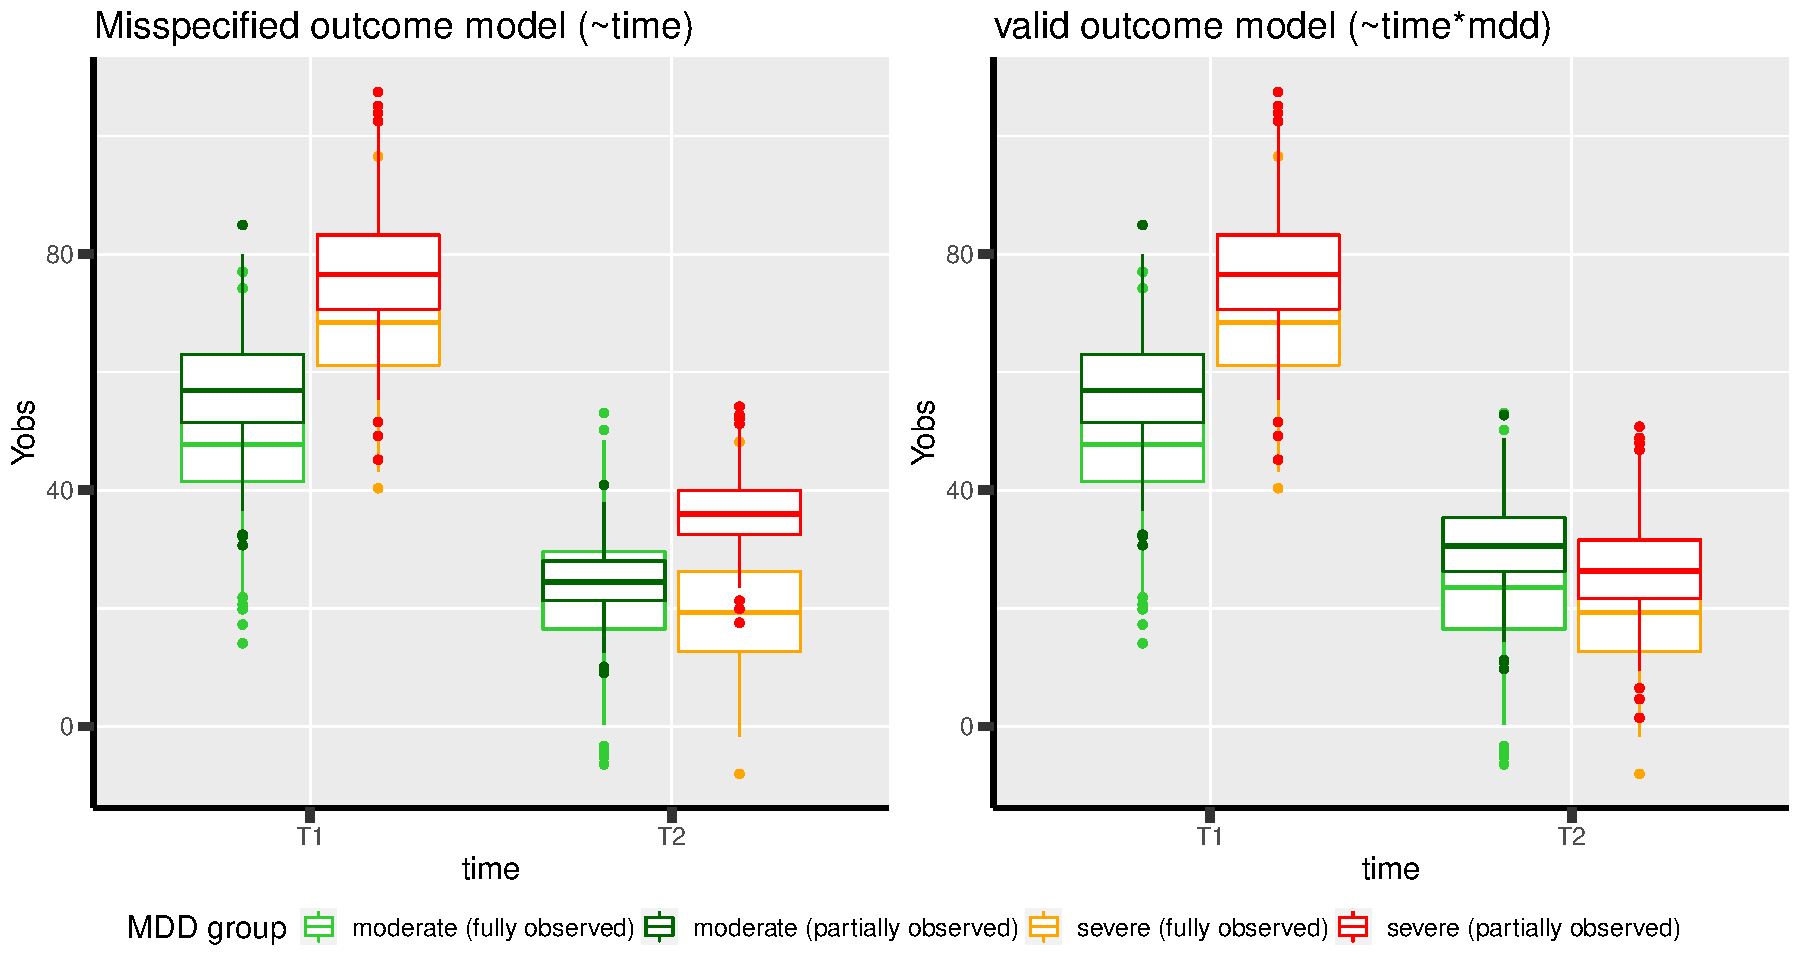
\includegraphics[width=\textwidth]{./figures/gg-imputationModel.pdf}
\caption{\label{fig:imputationModel}Distribution of the observed and imputed value when using the mixed model.}
\end{figure}

With a correct model for the outcome (i.e. adding the interaction),
the mixed would be able to impute the observations in an unbiased way:
\lstset{language=r,label= ,caption= ,captionpos=b,numbers=none}
\begin{lstlisting}
e.BFIoracle <- lme(Yobs~time*mdd, random = ~1|id, data = dtL.B,
                   na.action = na.omit)
summary(e.BFIoracle)$tTable
\end{lstlisting}

\begin{verbatim}
                     Value Std.Error   DF    t-value       p-value
(Intercept)       50.14399 0.3201715 1998  156.61602  0.000000e+00
timeT2           -24.97957 0.2351254 1029 -106.23938  0.000000e+00
mddsevere         24.51004 0.4527909 1998   54.13102  0.000000e+00
timeT2:mddsevere -24.90905 0.4443197 1029  -56.06111 4.849765e-315
\end{verbatim}


which would lead to a much better estimator:
\lstset{language=r,label= ,caption= ,captionpos=b,numbers=none}
\begin{lstlisting}
library(multcomp)
glht(e.BFIoracle, linfct = "timeT2+0.5*timeT2:mddsevere=0")
\end{lstlisting}

\begin{verbatim}

	 General Linear Hypotheses

Linear Hypotheses:
                                     Estimate
timeT2 + 0.5 * timeT2:mddsevere == 0   -37.43
\end{verbatim}



\bigskip

An alternative approach that does not require to specify an outcome
model is to use IPCW. It instead requires to correctly specify a model
for the probability of not dropping out at follow-up:
\lstset{language=r,label= ,caption= ,captionpos=b,numbers=none}
\begin{lstlisting}
dtW.B$observed <- !is.na(dtW.B$T2)
e.glmW.B <- glm(observed ~ T1, data = dtW.B,
                family = binomial(link = "logit"))
coef(e.glmW.B)
\end{lstlisting}

\begin{verbatim}
(Intercept)          T1 
  6.6357425  -0.1047988
\end{verbatim}


and then compute the weights for observations with full data:
\lstset{language=r,label= ,caption= ,captionpos=b,numbers=none}
\begin{lstlisting}
dtW.B$weight.oracle <- 1/predict(e.glmW.B, newdata = dtW.B,
                                 type = "response")
dtW.B[observed == TRUE, sum(weight.oracle)]
\end{lstlisting}

\begin{verbatim}
[1] 2045.06
\end{verbatim}


Note that the weights almost sum to the total sample size. We then
perform the complete case analysis with these weights:
\lstset{language=r,label= ,caption= ,captionpos=b,numbers=none}
\begin{lstlisting}
dtW.BCC <- dtW.B[!is.na(diff)]
e.BIPCW <- lm(diff~1, data = dtW.BCC, weights = dtW.BCC$weight.oracle)
summary(e.BIPCW)$coef
\end{lstlisting}

\begin{verbatim}
             Estimate Std. Error   t value Pr(>|t|)
(Intercept) -37.84241  0.4369635 -86.60314        0
\end{verbatim}


which gives a result very close to the true value. Here the IPCW works
very well because we have specified the correct censoring model.

\clearpage

\subsection{Illustrative example 2}
\label{sec:orgf578993}

Consider a similar study with a different cause of drop-out. This time
drop-out is not due to baseline value but due to the severity of the
disease (i.e. group): two patients severely depressed but with
different baseline score will have exactly the same probability of
drop-out while two patients, one severely depressed and the other
moderately depressed, with same baseline score will have different
probability of drop-out.

\bigskip

We can simulate such a dataset using the following function:
\lstset{language=r,label= ,caption= ,captionpos=b,numbers=none}
\begin{lstlisting}
set.seed(10)
dtL.L <- simTrialC(n = 1000, rho = 0.8, dmu = c(25,50),
                   causeC = "latent", piC = c(0.2,0.7))
print(dtL.L)
\end{lstlisting}

\begin{verbatim}
        id      mdd time        Y dropout     Yobs
   1:    1 moderate   T1 49.34367       0 49.34367
   2:    1 moderate   T2 23.43583       0 23.43583
   3:    2 moderate   T1 35.05489       0 35.05489
   4:    2 moderate   T2 13.50810       0 13.50810
   5:    3 moderate   T1 54.37770       0 54.37770
  ---                                             
3996: 1998   severe   T2 26.26605       1       NA
3997: 1999   severe   T1 70.81751       0 70.81751
3998: 1999   severe   T2 15.46369       1       NA
3999: 2000   severe   T1 73.53750       0 73.53750
4000: 2000   severe   T2 23.75026       1       NA
\end{verbatim}

Overall the expected treatment effect is the same as before and,
without drop-out, the linear model gives the same estimates:
\lstset{language=r,label= ,caption= ,captionpos=b,numbers=none}
\begin{lstlisting}
dtW.Loracle <- dcast(dtL.L, formula = id ~ time, value.var = "Y")
dtW.Loracle$diff <- dtW.Loracle$T2-dtW.Loracle$T1
e.Loracle <- lm(diff~1, data = dtW.Loracle)
summary(e.Loracle)$coef
\end{lstlisting}

\begin{verbatim}
             Estimate Std. Error   t value Pr(>|t|)
(Intercept) -37.34478  0.3131657 -119.2492        0
\end{verbatim}


\clearpage

With drop-out, a complete case analysis would still lead to a downward
biased estimator:
\lstset{language=r,label= ,caption= ,captionpos=b,numbers=none}
\begin{lstlisting}
dtW.L <- dcast(dtL.L, formula = id + mdd ~ time, value.var = "Yobs")
dtW.L$diff <- dtW.L$T2-dtW.L$T1
dtW.LCC <- dtW.L[!is.na(diff)]
e.LCC <- lm(diff~1, data = dtW.LCC)
summary(e.LCC)$coef
\end{lstlisting}

\begin{verbatim}
             Estimate Std. Error   t value Pr(>|t|)
(Intercept) -31.47144  0.3853402 -81.67182        0
\end{verbatim}


for a reason similar as before, as patients from the severely
depressed group will drop more often and they benefit more from the
treatmet. We can use a linear mixed model (i.e. full information):
\lstset{language=r,label= ,caption= ,captionpos=b,numbers=none}
\begin{lstlisting}
require(nlme)
e.LFI <- lme(Yobs~time, random = ~1|id, data = dtL.L, na.action = na.omit)
summary(e.LFI)$tTable
\end{lstlisting}

\begin{verbatim}
                Value Std.Error   DF   t-value p-value
(Intercept)  62.39901 0.3216035 1999 194.02463       0
timeT2      -33.90248 0.3789931 1090 -89.45409       0
\end{verbatim}

which is better than the complete case analysis still biased because
once more the outcome model is misspecified. With a correctly
specified outcome model, we would get a much better estimate:
\lstset{language=r,label= ,caption= ,captionpos=b,numbers=none}
\begin{lstlisting}
e.LFIoracle <- lme(Yobs~time*mdd, random = ~1|id, data = dtL.L, na.action = na.omit)
glht(e.LFIoracle, linfct = "timeT2+0.5*timeT2:mddsevere=0")

\end{lstlisting}

\begin{verbatim}

	 General Linear Hypotheses

Linear Hypotheses:
                                     Estimate
timeT2 + 0.5 * timeT2:mddsevere == 0    -37.3
\end{verbatim}


\bigskip

 When using IPCW, we should model the probability of not dropping out
at follow-up as a function of the latent group:
\lstset{language=r,label= ,caption= ,captionpos=b,numbers=none}
\begin{lstlisting}
dtW.L$observed <- !is.na(dtW.L$T2)
e.glmW.Loracle <- glm(observed ~ mdd, data = dtW.L,
                     family = binomial(link = "logit"))
\end{lstlisting}

and then compute the weights for observations with full data:
\lstset{language=r,label= ,caption= ,captionpos=b,numbers=none}
\begin{lstlisting}
dtW.L$weight.oracle <- 1/predict(e.glmW.Loracle, newdata = dtW.L,type = "response")
dtW.L[observed == TRUE, sum(weight.oracle)]
\end{lstlisting}

\begin{verbatim}
[1] 2000
\end{verbatim}


Note that the weights sum to the total sample size. We then perform
the complete case analysis with these weights:
\lstset{language=r,label= ,caption= ,captionpos=b,numbers=none}
\begin{lstlisting}
dtW.LCC <- dtW.L[!is.na(diff)]
e.LIPCWoracle <- lm(diff~1, data = dtW.LCC, weights = dtW.LCC$weight.oracle)
summary(e.LIPCWoracle)$coef
\end{lstlisting}

\begin{verbatim}
             Estimate Std. Error  t value Pr(>|t|)
(Intercept) -37.35191  0.4242621 -88.0397        0
\end{verbatim}


which gives a result very close to the true value. A more feasible
IPCW would use the baseline score to define the weights:
\lstset{language=r,label= ,caption= ,captionpos=b,numbers=none}
\begin{lstlisting}
e.glmW.L <- glm(observed ~ T1, data = dtW.L,
              family = binomial(link = "logit"))
dtW.L$weight <- 1/predict(e.glmW.L, newdata = dtW.L, type = "response")
dtW.L[observed == TRUE, sum(weight)]
\end{lstlisting}

\begin{verbatim}
[1] 2038.825
\end{verbatim}


We then perform the complete case analysis with these new weights:
\lstset{language=r,label= ,caption= ,captionpos=b,numbers=none}
\begin{lstlisting}
dtW.LCC <- dtW.L[!is.na(diff)]
e.LIPCW <- lm(diff~1, data = dtW.LCC, weights = dtW.LCC$weight)
summary(e.LIPCW)$coef
\end{lstlisting}

\begin{verbatim}
            Estimate Std. Error   t value Pr(>|t|)
(Intercept) -36.0517  0.4258783 -84.65258        0
\end{verbatim}


\clearpage

\subsection{Simulation study}
\label{sec:org2e65e9f}

The quality of the previous estimators is compared using a simulation
study (see appendix \ref{SM:dataAnalysis}):
\begin{itemize}
\item first under the right generative model (i.e. multivariate normal distribution)
\item then under alternative generative models (i.e multivariate
t-distribution or Gaussian copula with margins contaminated by a
Gamma or uniform distribution). Indeed it is believed that the LMM
in presence of missing value is not robustness to parametric
assumptions, i.e. lead to biased results for certain non-normal
distributions. Some simulations studies support this point
\citep{lu2009impact}.
\end{itemize}

\subsubsection{Valid parametric assumptions}
\label{sec:orga033992}

Here is an example of result on a single trial subject to 3 different
drop-out mechanisms:
\lstset{language=r,label= ,caption= ,captionpos=b,numbers=none}
\begin{lstlisting}
warper3TrialC(n = 1000, rho = 0.8, dmu = c(25,50),
              piC = list(0.5,1,c(0.2,0.7)), short = TRUE, seed = 10)
\end{lstlisting}

\begin{verbatim}
     causeC dropout rho    n dmu         model  estimate        se  statistic p.value seed
1    random  0.4805 0.8 1000  25        oracle -37.34478 0.3131657 -119.24924       0   10
2                                complete case -37.60385 0.4396445  -85.53240       0     
3                                    FI.oracle -37.47880 0.1997909 -187.59009       0     
4                                           FI -37.65209 0.4239748  -88.80738       0     
5                                  IPCW.oracle -37.60385 0.4396445  -85.53240       0     
6  baseline  0.4845 0.8 1000  25        oracle -37.34478 0.3131657 -119.24924       0   10
7                                complete case -30.98307 0.3889309  -79.66214       0     
8                                    FI.oracle -37.43410 0.2221598 -168.50078       0     
9                                           FI -34.72139 0.3922185  -88.52563       0     
10                                 IPCW.oracle -37.84241 0.4369635  -86.60314       0     
11   latent  0.4545 0.8 1000  25        oracle -37.34478 0.3131657 -119.24924       0   10
12                               complete case -31.47144 0.3853402  -81.67182       0     
13                                   FI.oracle -37.30128 0.2145794 -173.83442       0     
14                                          FI -33.90249 0.3789936  -89.45400       0     
15                                 IPCW.oracle -37.35191 0.4242621  -88.03970       0     
16                                        IPCW -36.05170 0.4258783  -84.65258       0
\end{verbatim}

Replicating a 1000 times and also varying the correlation coefficient leads to:
\lstset{language=r,label= ,caption= ,captionpos=b,numbers=none}
\begin{lstlisting}
dt.simGaussian <- warper3TrialC(n = 1000, n.rep = 1000, cl = 50,
                                rho = c(0,0.25,0.5,0.8),
                                dmu = c(25,50),
                                piC = list(0.5,1,c(0.2,0.7)),
                                short = FALSE, seed = 10)
\end{lstlisting}

\clearpage

\lstset{language=r,label= ,caption= ,captionpos=b,numbers=none}
\begin{lstlisting}
gg.simGaussian <- ggSimRes(dt.simGaussian)
\end{lstlisting}

\begin{figure}[!h]
\centering
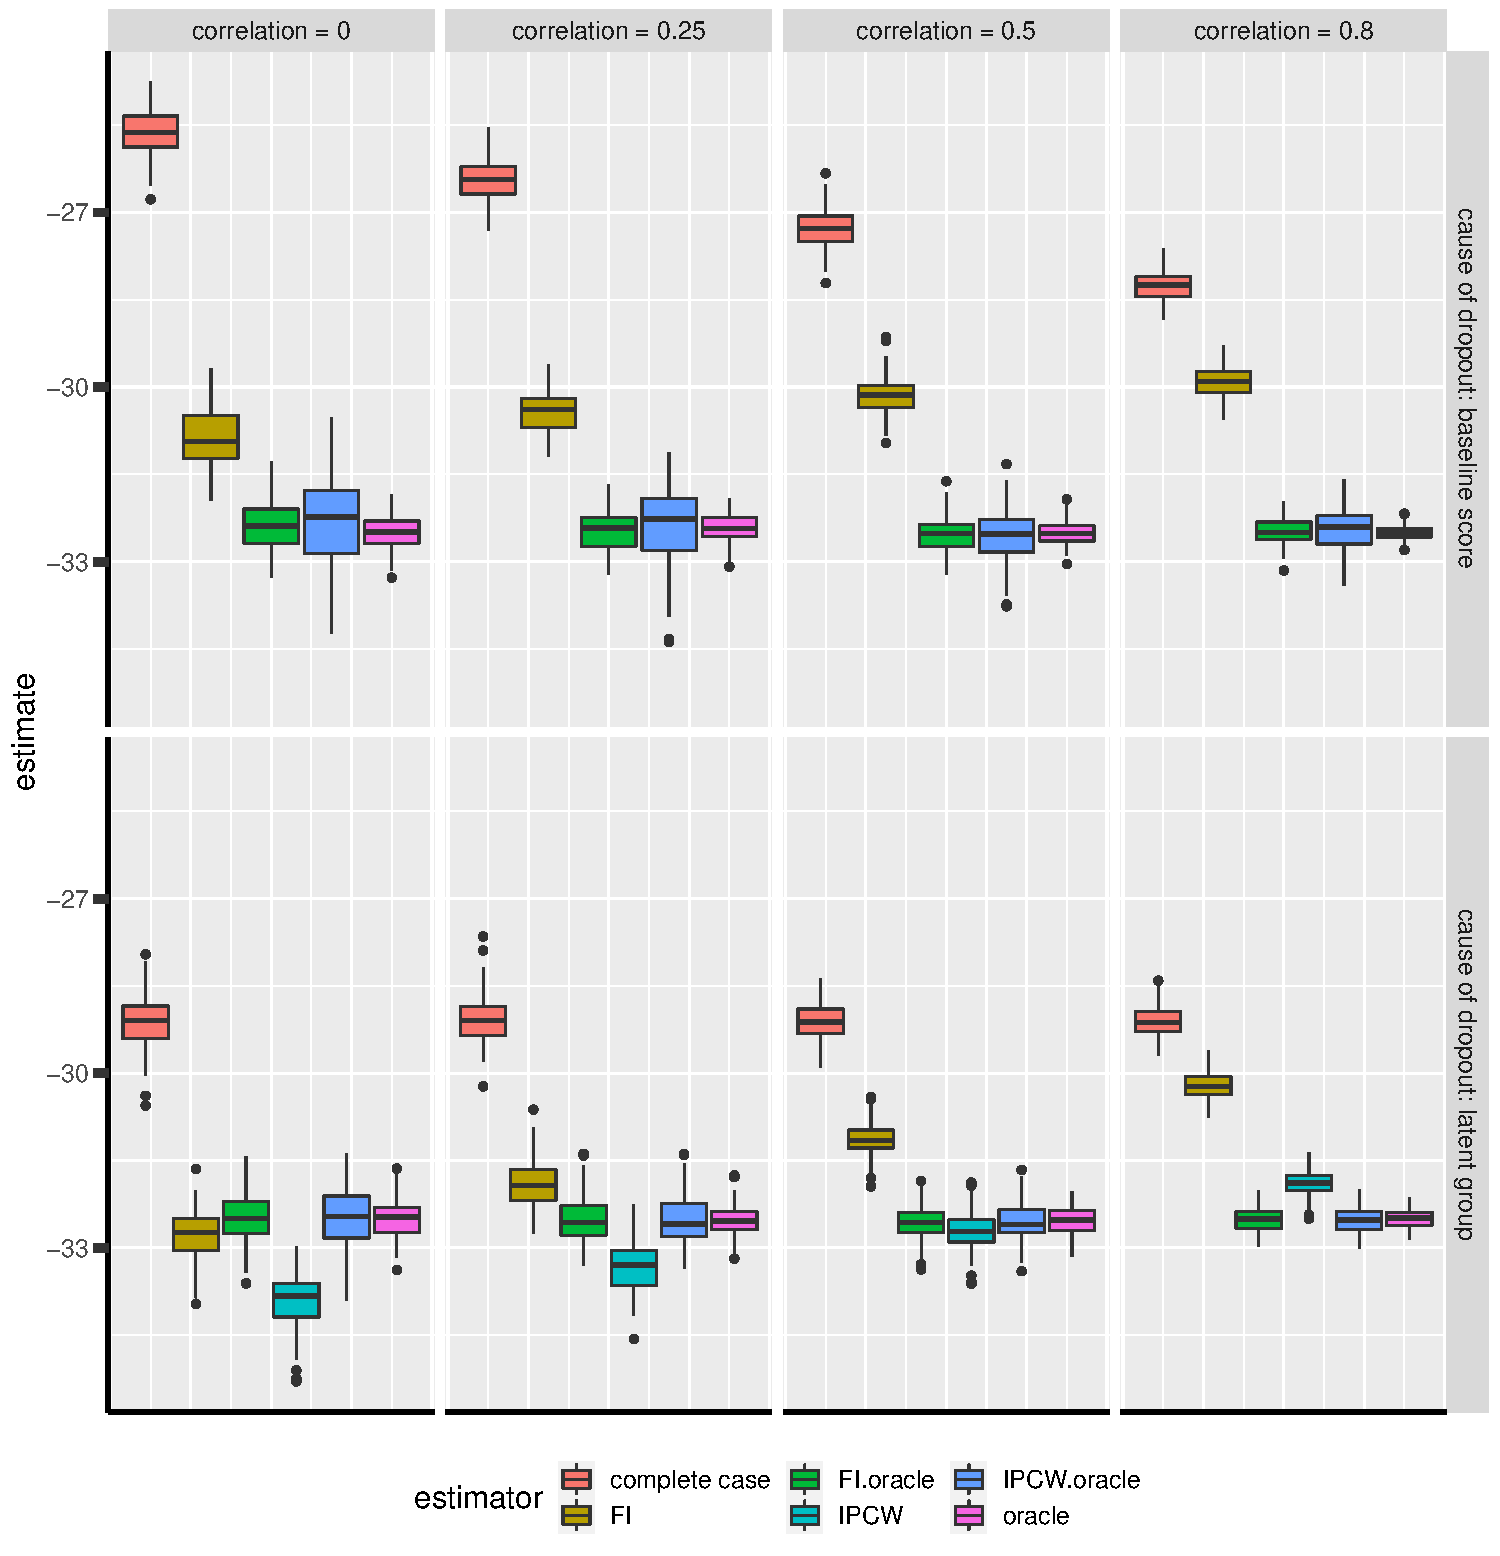
\includegraphics[width=\textwidth]{./figures/simStudy-bias.pdf}
\caption{\label{fig:simulationGaussian}Comparison between the empirical distributions of the estimators (Gaussian case) for a sample size of 1000 using 1000 datasets. FI: full information (random intercept model), IPCW: inverse probability of censoring weights.}
\end{figure}

\clearpage

\subsubsection{Incorrect parametric assumptions - heavy tails}
\label{sec:org6c08a2e}

Data were simulated using a student distribution with 3 degrees of
freedom. See figure below for an example:
\begin{figure}[!h]
\centering
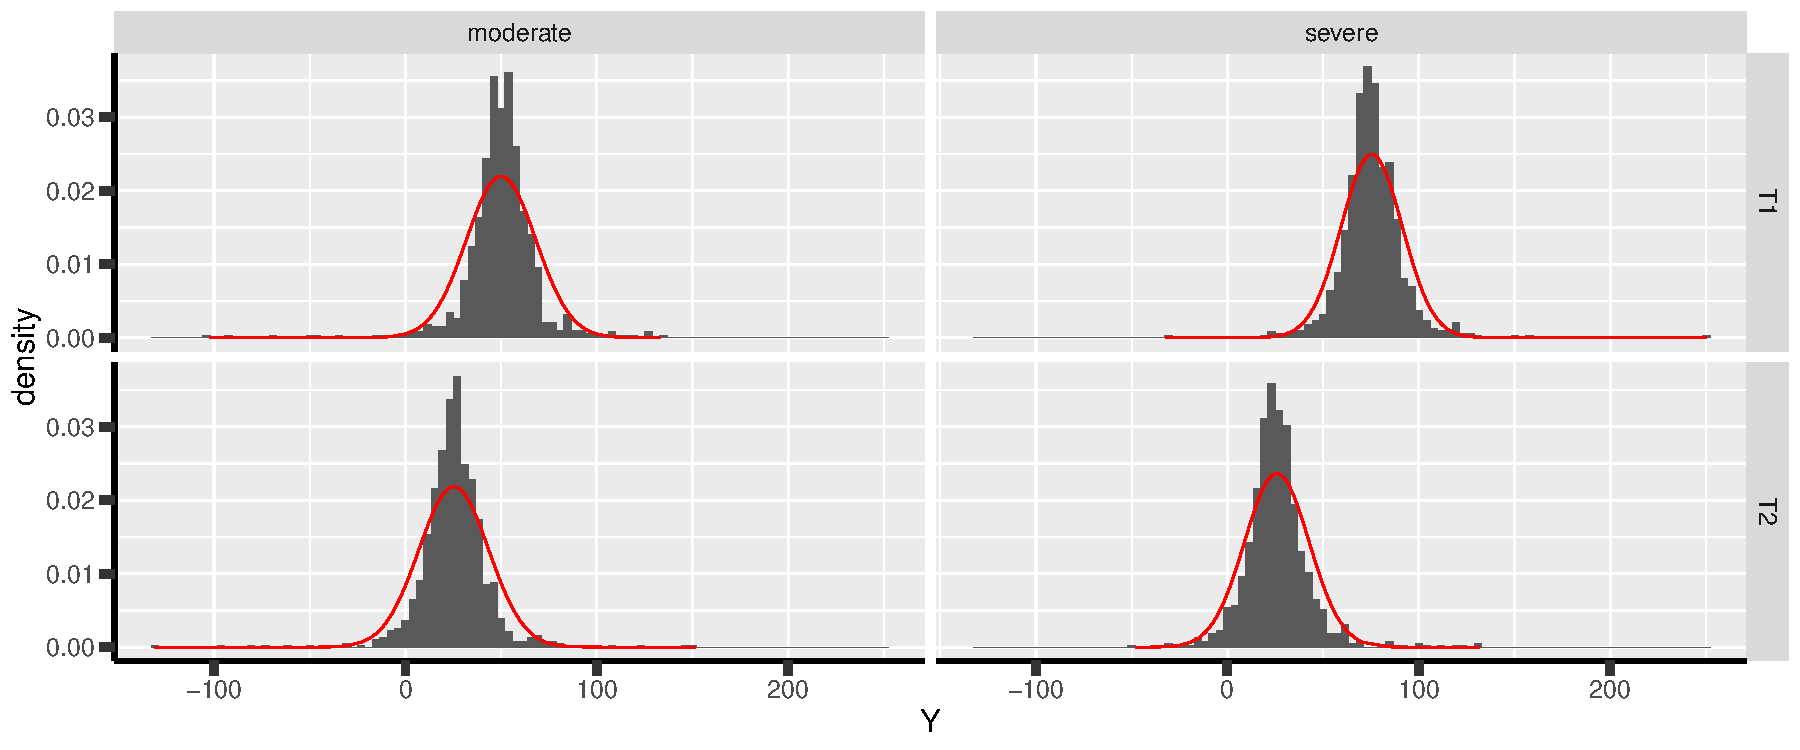
\includegraphics[trim={0 0 0 0},width=1\textwidth]{./figures/simStudy-student-hist.pdf}
\caption{\label{fig:student-hist}Histogram of the simulated outcome for one study when using a multivariate student distribution. The red line indicates the best fitting Gaussian distribution.}
\end{figure}

Here is an example of result on a single trial subject to 3 different
drop-out mechanisms:
\lstset{language=r,label= ,caption= ,captionpos=b,numbers=none}
\begin{lstlisting}
warper3TrialC(n = 1000, rho = 0.8, dmu = c(25,50),
              piC = list(0.5,1,c(0.2,0.7)), df = 3,
              short = TRUE, seed = 10)
\end{lstlisting}

\begin{verbatim}
     causeC dropout rho    n dmu         model  estimate        se  statistic p.value seed
1    random   0.499 0.8 1000  25        oracle -37.14393 0.3679432 -100.95019       0   10
2                                complete case -37.16037 0.4952641  -75.03142       0     
3                                    FI.oracle -37.29110 0.3111914 -119.83333       0     
4                                           FI -37.11295 0.4800798  -77.30579       0     
5                                  IPCW.oracle -37.16037 0.4952641  -75.03142       0     
6  baseline   0.501 0.8 1000  25        oracle -37.14393 0.3679432 -100.95019       0   10
7                                complete case -30.92928 0.4931273  -62.72067       0     
8                                    FI.oracle -37.80839 0.3675489 -102.86630       0     
9                                           FI -34.64776 0.4886764  -70.90122       0     
10                                 IPCW.oracle -38.33936 0.5234635  -73.24172       0     
11   latent  0.4405 0.8 1000  25        oracle -37.14393 0.3679432 -100.95019       0   10
12                               complete case -31.75154 0.4764017  -66.64867       0     
13                                   FI.oracle -37.55087 0.3591784 -104.54658       0     
14                                          FI -33.55264 0.4642002  -72.28053       0     
15                                 IPCW.oracle -37.55106 0.5001728  -75.07618       0     
16                                        IPCW -34.37854 0.5064666  -67.87919       0
\end{verbatim}

Replicating a 1000 times and also varying the correlation coefficient leads to:
\lstset{language=r,label= ,caption= ,captionpos=b,numbers=none}
\begin{lstlisting}
dt.simStudent <- warper3TrialC(n = 1000, n.rep = 1000, cl = 50,
                               rho = c(0,0.25,0.5,0.8),
                               dmu = c(25,50), df = 3,
                               piC = list(0.5,1,c(0.2,0.7)), 
                               short = FALSE, seed = 10)
\end{lstlisting}

\begin{figure}[!h]
\centering
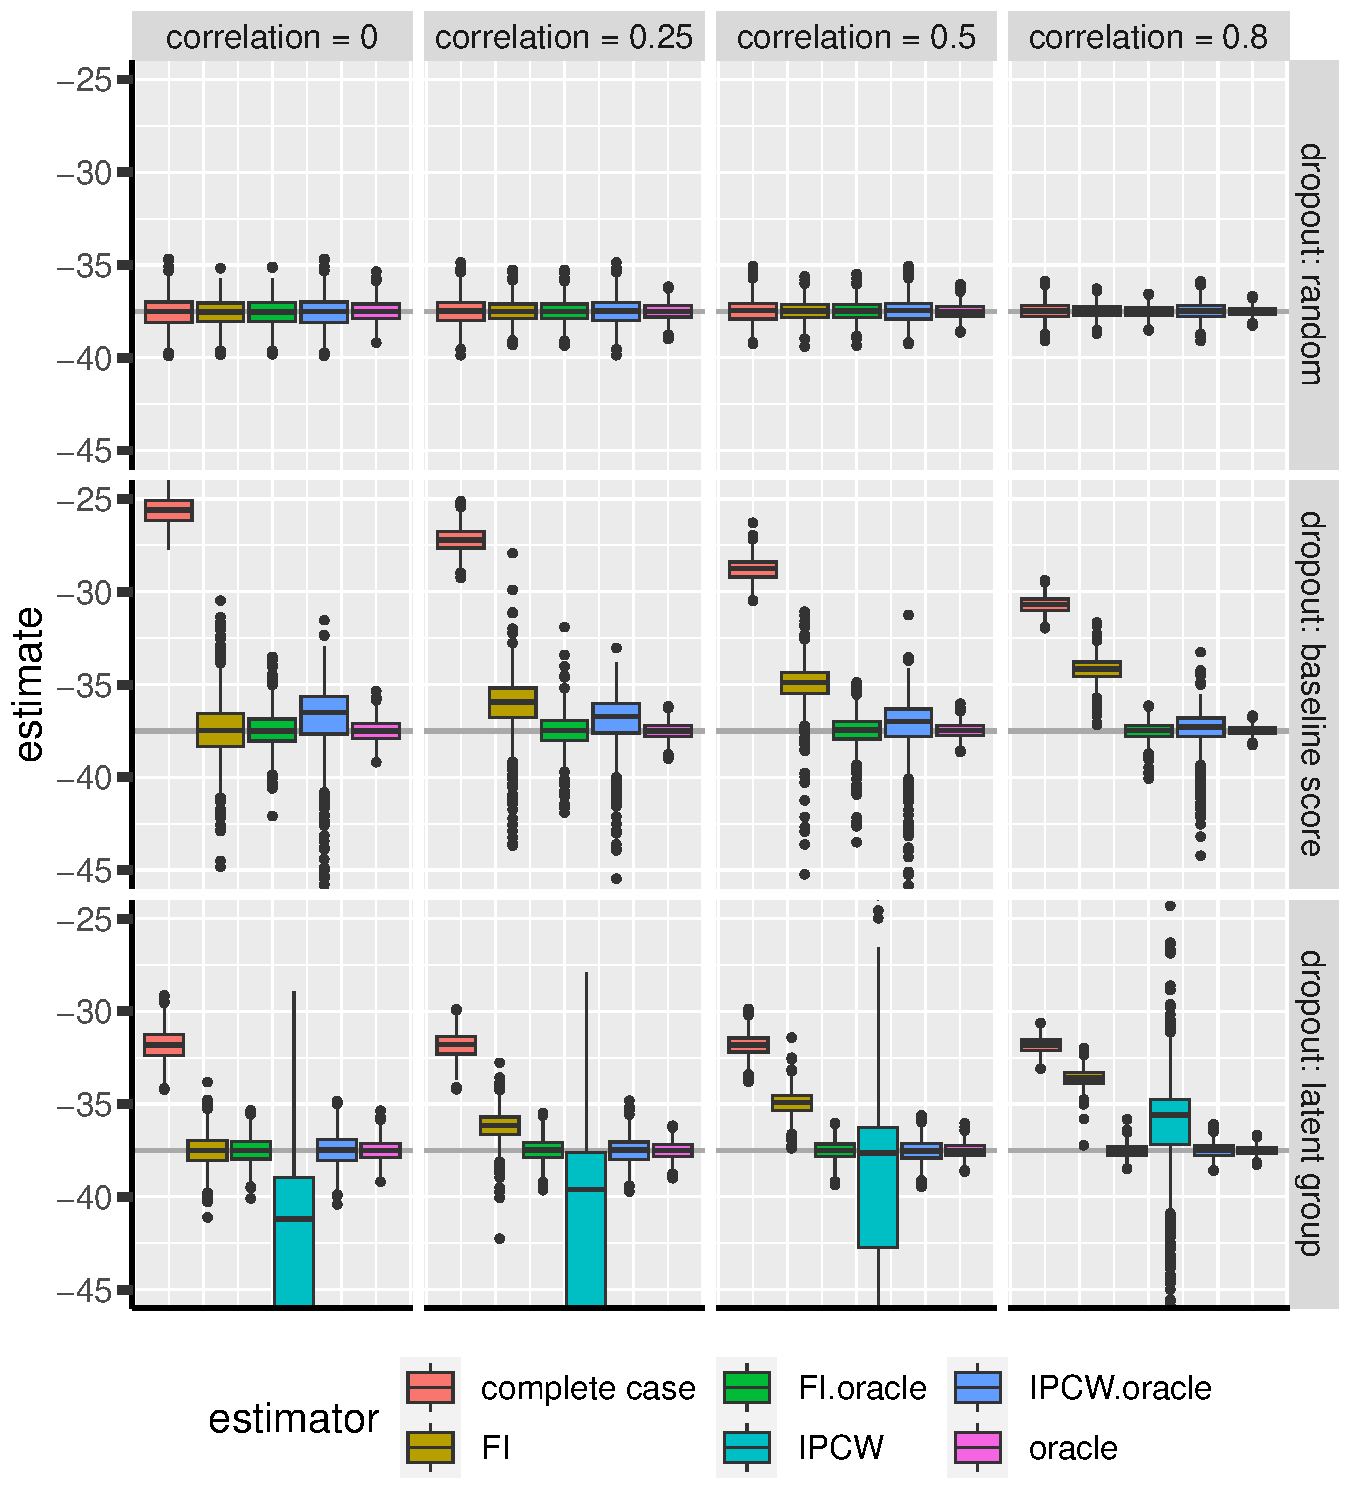
\includegraphics[width=\textwidth]{./figures/simStudy-bias-t3.pdf}
\caption{\label{fig:simulationGaussian}Comparison between the empirical distributions of the estimators (Studence case) for a sample size of 1000 using 1000 datasets. FI: full information (random intercept model), IPCW: inverse probability of censoring weights.}
\end{figure}

\clearpage

\subsubsection{Incorrect parametric assumptions - skewed}
\label{sec:orgaba7b8b}


Data were simulated as in the correctly specific case but a a gamma
noise added with shape parameter 1 and scale parameter 20. See
figure below for an example:
\begin{figure}[!h]
\centering
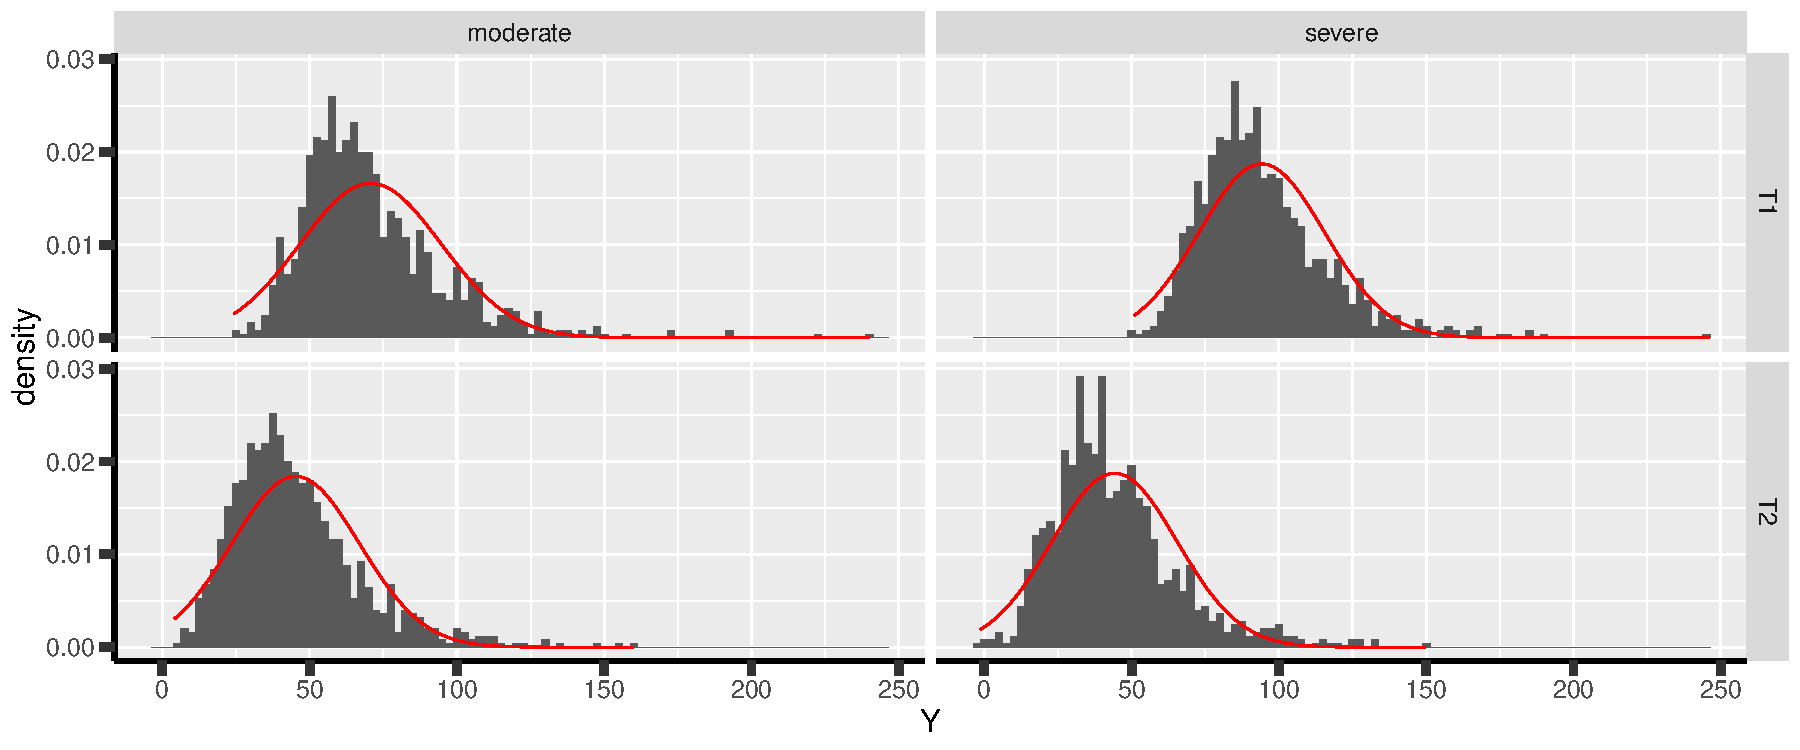
\includegraphics[trim={0 0 0 0},width=1\textwidth]{./figures/simStudy-gamma-hist.pdf}
\caption{\label{fig:student-hist}Histogram of the simulated outcome for one study when using a multivariate normal distribution with added gamma distributed noise. The red line indicates the best fitting Gaussian distribution.}
\end{figure}

Here is an example of result on a single trial subject to 3 different
drop-out mechanisms:
\lstset{language=r,label= ,caption= ,captionpos=b,numbers=none}
\begin{lstlisting}
warper3TrialC(n = 1000, rho = 0.8, dmu = c(25,50),
              piC = list(0.5,1,c(0.2,0.7)), gamma = c(1,20),
              short = TRUE, seed = 10)
\end{lstlisting}

\begin{verbatim}
     causeC dropout rho    n dmu         model  estimate        se statistic       p.value seed
1    random  0.4985 0.8 1000  25        oracle -37.71493 0.6920647 -54.49625  0.000000e+00   10
2                                complete case -36.84023 1.0198759 -36.12227 1.229736e-183     
3                                    FI.oracle -37.08504 0.8243480 -44.98712  0.000000e+00     
4                                           FI -37.04004 0.9064410 -40.86315  0.000000e+00     
5                                  IPCW.oracle -36.84023 1.0198759 -36.12227 1.229736e-183     
6  baseline   0.731 0.8 1000  25        oracle -37.71493 0.6920647 -54.49625  0.000000e+00   10
7                                complete case -18.62851 1.0242595 -18.18729  6.030064e-58     
8                                    FI.oracle -35.42771 1.1314386 -31.31210  0.000000e+00     
9                                           FI -32.20733 1.0480515 -30.73068  0.000000e+00     
10                                 IPCW.oracle -31.92106 1.0882540 -29.33236 1.324571e-113     
11   latent    0.45 0.8 1000  25        oracle -37.71493 0.6920647 -54.49625  0.000000e+00   10
12                               complete case -32.20863 0.9352860 -34.43720 7.110637e-177     
13                                   FI.oracle -37.68618 0.8512623 -44.27093  0.000000e+00     
14                                          FI -36.49446 0.8547891 -42.69411  0.000000e+00     
15                                 IPCW.oracle -38.15756 0.9137801 -41.75792 4.877840e-229     
16                                        IPCW -39.57164 1.1179406 -35.39691 8.854345e-184
\end{verbatim}

Replicating a 1000 times and also varying the correlation coefficient leads to:
\lstset{language=r,label= ,caption= ,captionpos=b,numbers=none}
\begin{lstlisting}
gg.simGamma <- ggSimRes(dt.simGamma, ylim = c(-45, -25))
\end{lstlisting}

\begin{figure}[!h]
\centering
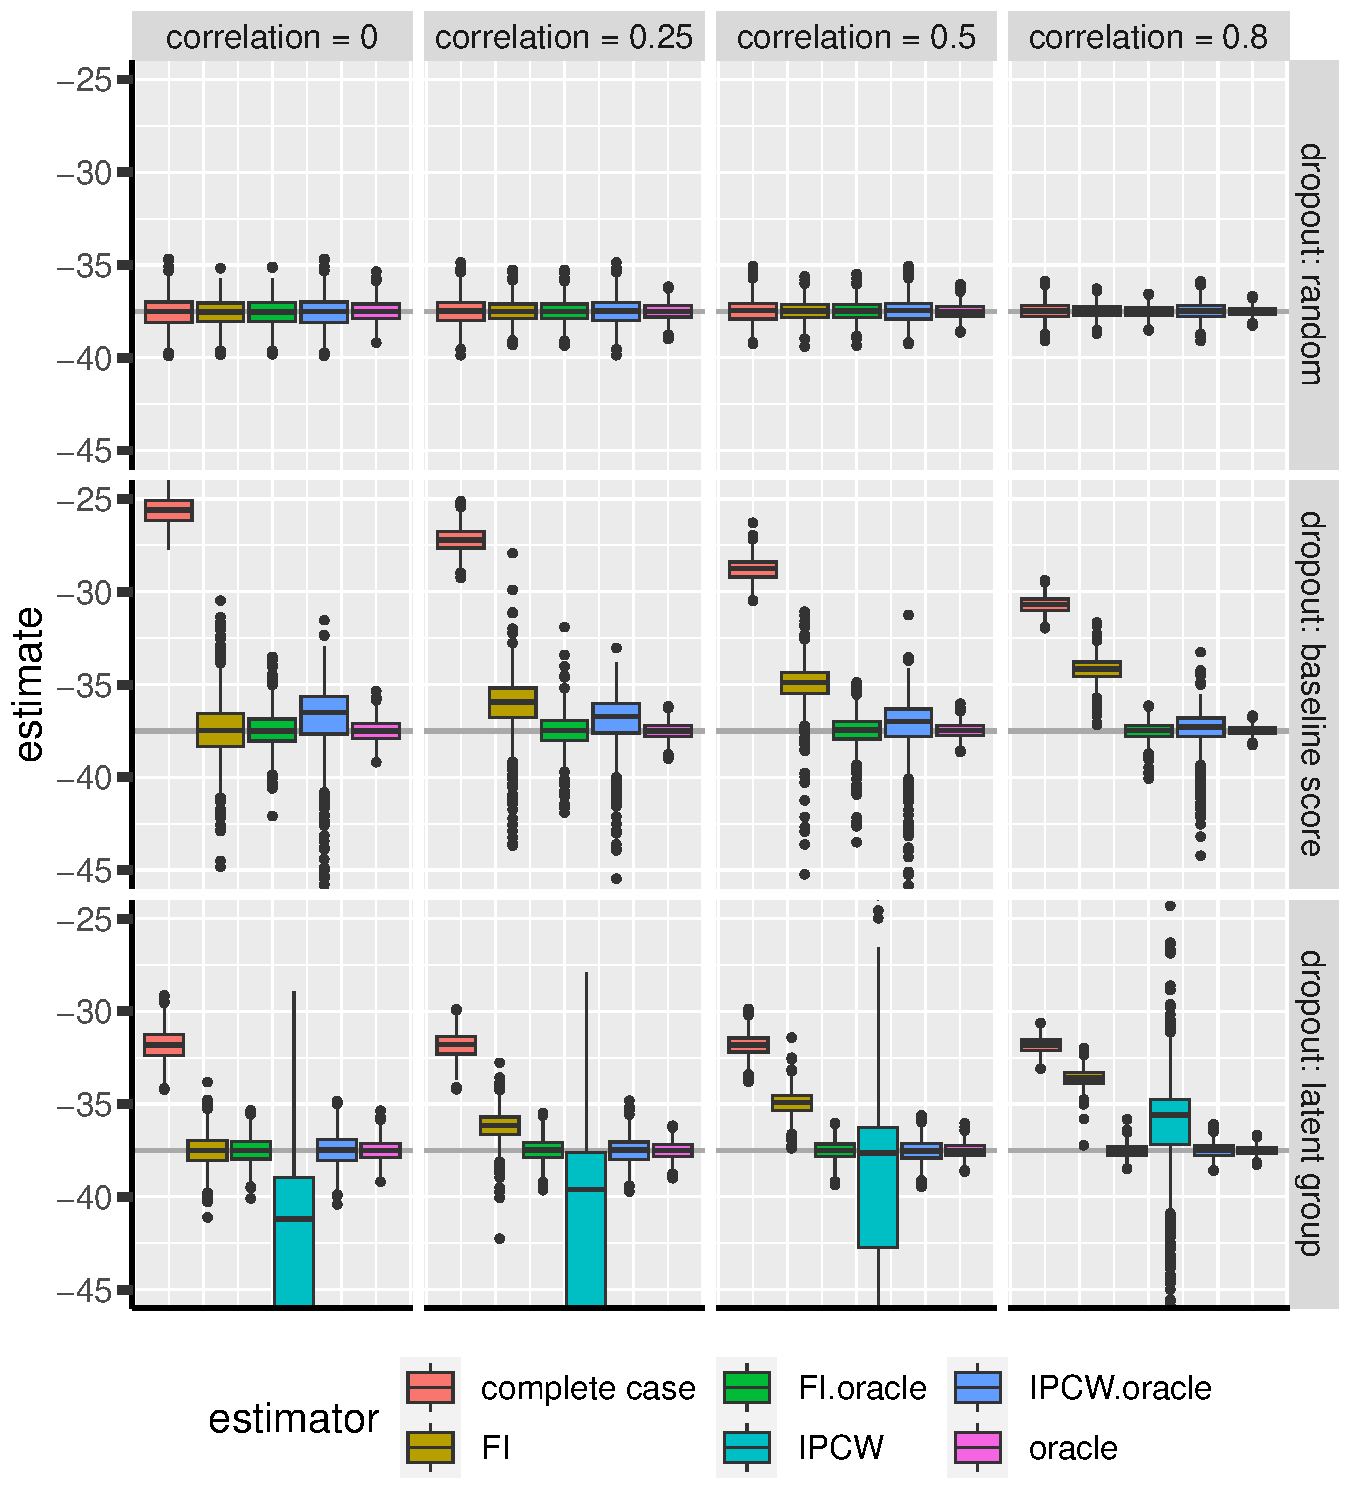
\includegraphics[width=\textwidth]{./figures/simStudy-bias-gamma.pdf}
\caption{\label{fig:simulationGaussian}Comparison between the empirical distributions of the estimators (Gamma case) for a sample size of 1000 using 1000 datasets. FI: full information (random intercept model), IPCW: inverse probability of censoring weights.}
\end{figure}

\clearpage

\subsubsection{Incorrect parametric assumptions - uniform}
\label{sec:org9d815a6}


Data were simulated as in the correctly specific case but with a
uniform noise added (min 0 and max 100). See figure below for an
example:
\begin{figure}[!h]
\centering
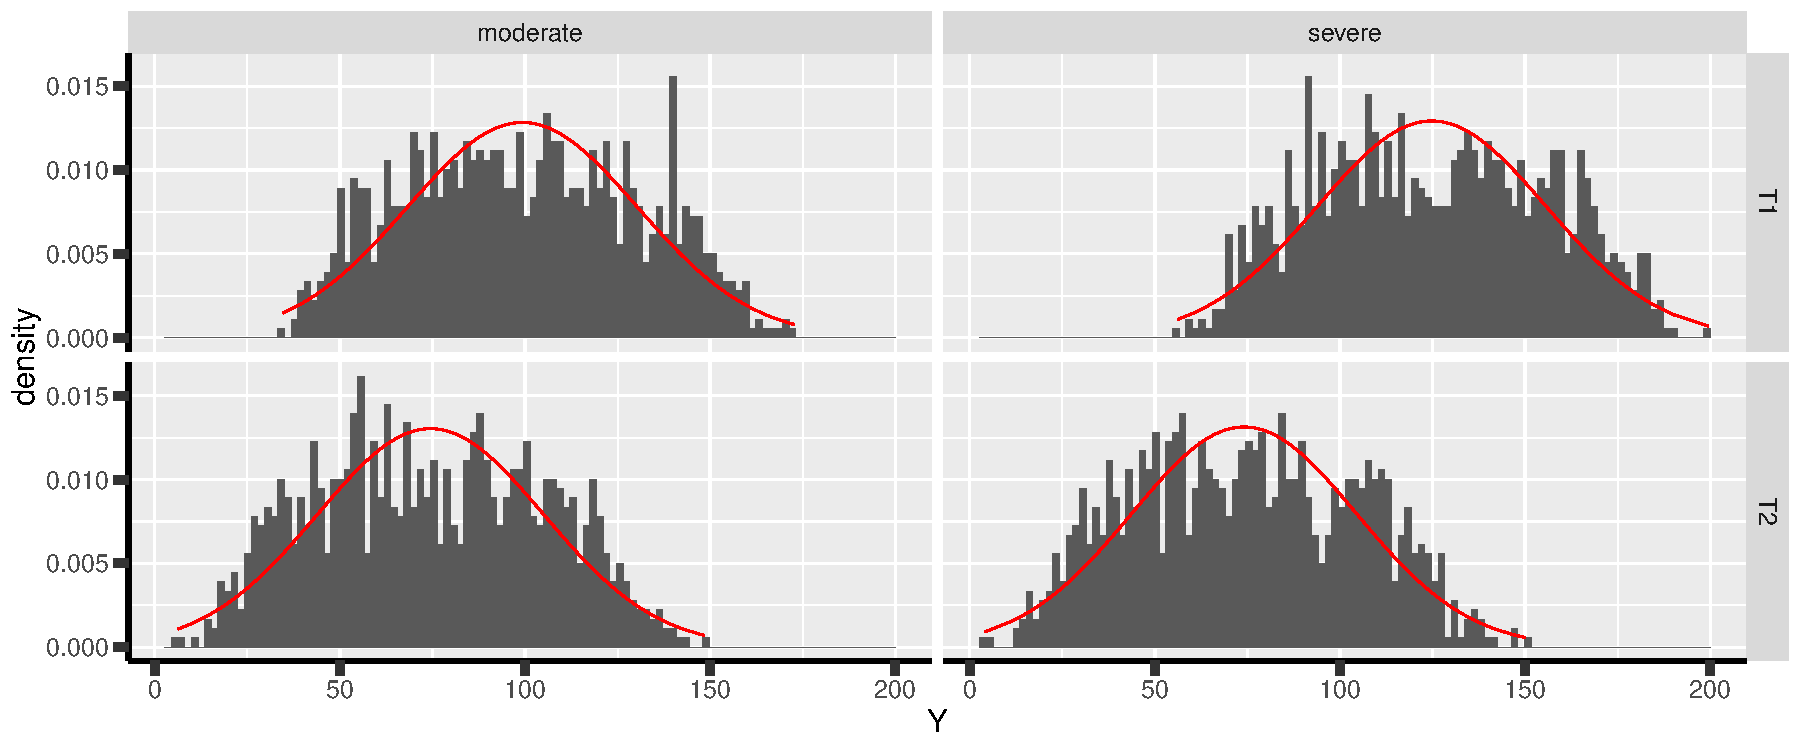
\includegraphics[trim={0 0 0 0},width=1\textwidth]{./figures/simStudy-unif-hist.pdf}
\caption{\label{fig:student-hist}Histogram of the simulated outcome for one study when using a multivariate normal distribution with added gamma distributed noise. The red line indicates the best fitting Gaussian distribution.}
\end{figure}


Here is an example of result on a single trial subject to 3 different
drop-out mechanisms:
\lstset{language=r,label= ,caption= ,captionpos=b,numbers=none}
\begin{lstlisting}
warper3TrialC(n = 1000, rho = 0.8, dmu = c(25,50),
              piC = list(0.5,0.2,c(0.2,0.7)), unif = c(0,100),
              short = TRUE, seed = 11)
\end{lstlisting}

\begin{verbatim}
     causeC dropout rho    n dmu         model  estimate        se statistic       p.value seed
1    random   0.501 0.8 1000  25        oracle -38.34944 0.9636263 -39.79700 1.397159e-255   11
2                                complete case -36.68859 1.3486849 -27.20323 2.480433e-122     
3                                    FI.oracle -37.25888 1.1481783 -32.45043  0.000000e+00     
4                                           FI -37.26851 1.2014576 -31.01941  0.000000e+00     
5                                  IPCW.oracle -36.68859 1.3486849 -27.20323 2.480433e-122     
6  baseline    0.72 0.8 1000  25        oracle -38.34944 0.9636263 -39.79700 1.397159e-255   11
7                                complete case -27.67410 1.8056059 -15.32677  1.607715e-44     
8                                    FI.oracle -40.92304 1.4750654 -27.74321  0.000000e+00     
9                                           FI -40.91608 1.5305085 -26.73365  0.000000e+00     
10                                 IPCW.oracle -40.17666 1.8218866 -22.05223  5.211715e-78     
11   latent   0.457 0.8 1000  25        oracle -38.34944 0.9636263 -39.79700 1.397159e-255   11
12                               complete case -32.17486 1.2989146 -24.77057 1.007704e-107     
13                                   FI.oracle -38.00854 1.2082477 -31.45757  0.000000e+00     
14                                          FI -37.00927 1.1717526 -31.58454  0.000000e+00     
15                                 IPCW.oracle -38.00831 1.3010987 -29.21248 7.049359e-139     
16                                        IPCW -36.89577 1.2986463 -28.41095 3.442202e-133
\end{verbatim}


Replicating a 1000 times and also varying the correlation coefficient leads to:
\lstset{language=r,label= ,caption= ,captionpos=b,numbers=none}
\begin{lstlisting}
dt.simUnif <- warper3TrialC(n = 1000, n.rep = 1000, cl = 50,
                            rho = c(0,0.25,0.5,0.8),
                            dmu = c(25,50), unif = c(0,100),
                            piC = list(0.5,0.2,c(0.2,0.7)), 
                            short = FALSE, seed = 10)
\end{lstlisting}


\begin{figure}[!h]
\centering
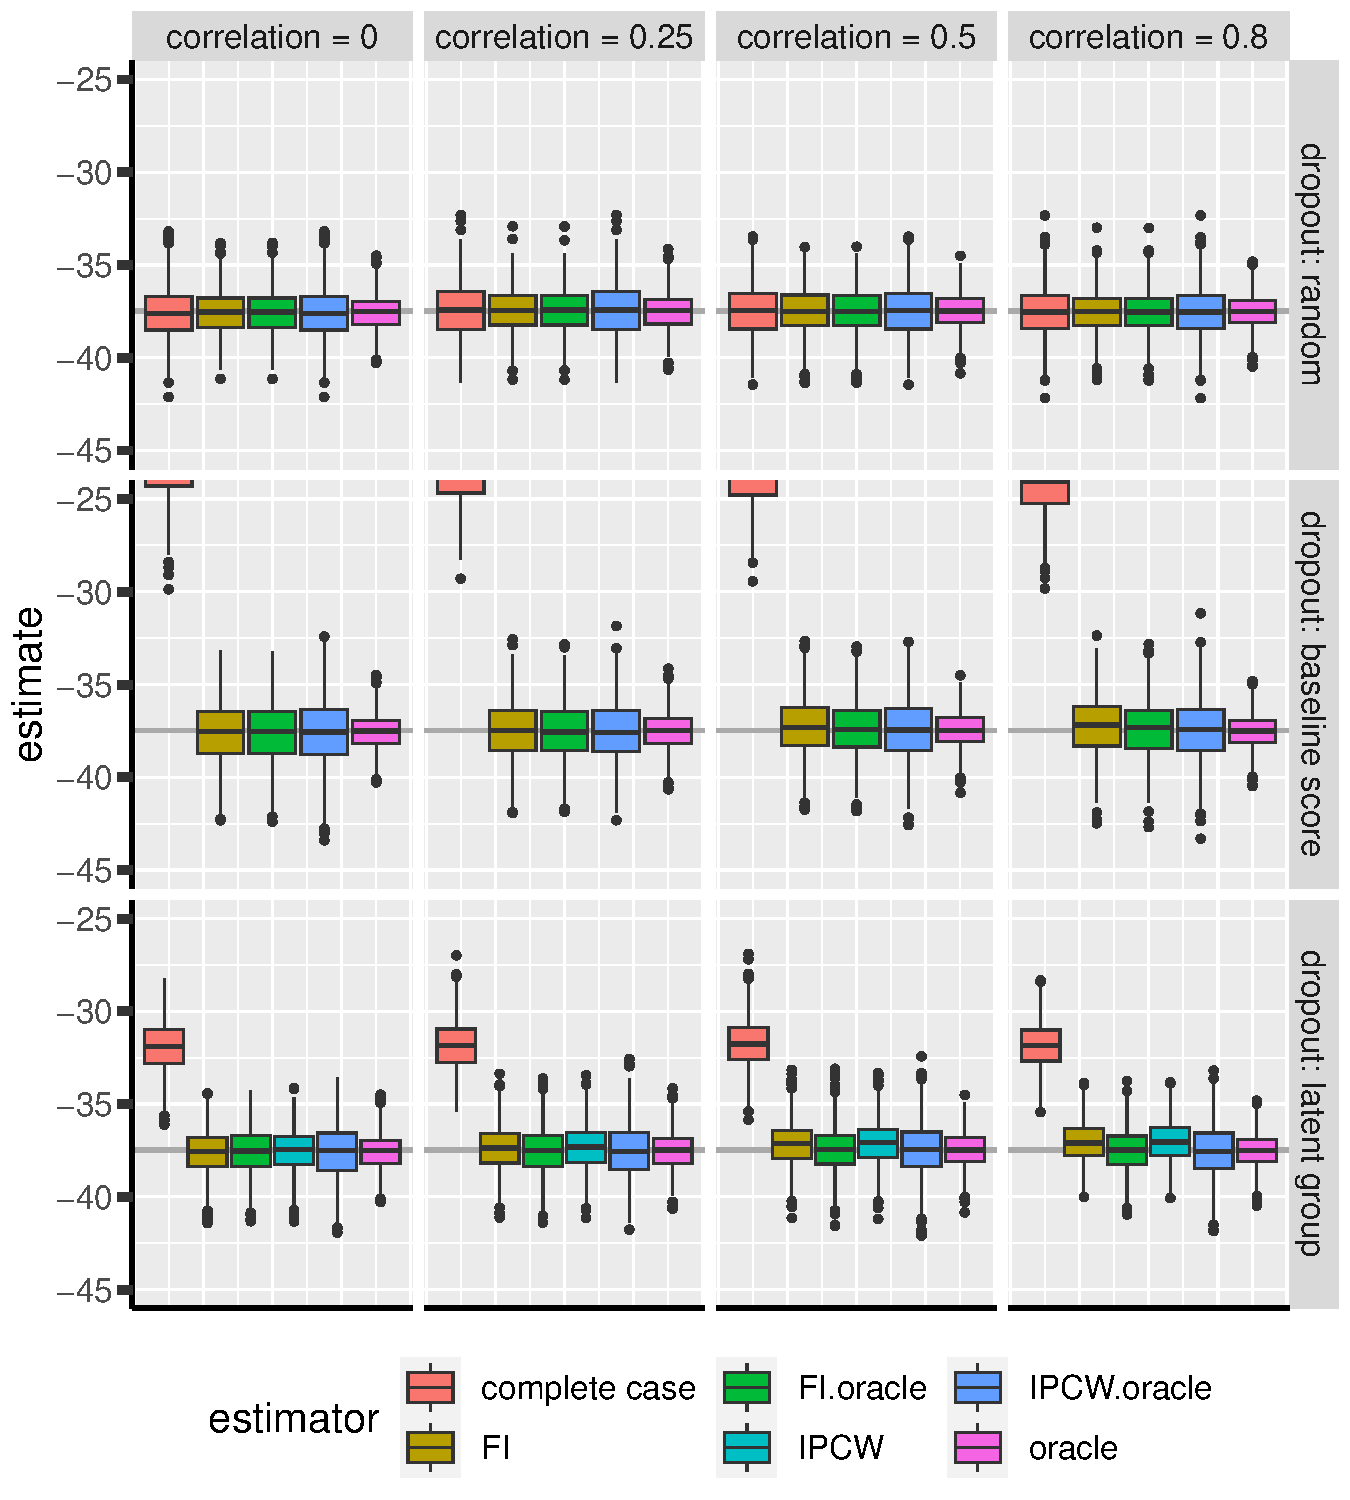
\includegraphics[width=\textwidth]{./figures/simStudy-bias-unif.pdf}
\caption{\label{fig:simulationGaussian}Comparison between the empirical distributions of the estimators (uniform case) for a sample size of 1000 using 1000 datasets. FI: full information (random intercept model), IPCW: inverse probability of censoring weights.}
\end{figure}


\clearpage

\section{Binary outcome}
\label{sec:orga607cf2}

\subsection{Illustrative example}
\label{sec:org8103a10}
A somehow similar approach can be used for binary endpoints. Consider
now a study comparing the survival probability at 1 year of patients
treated with a new drug vs. standard care. The population is composed
of two types of patients, say some with hypertension and some
without. Survival as well as the treatment effect may differ depending
of the hypertension status. Hypertension may also affect the drop-out
probability.

\bigskip

We can simulate such a dataset using the following function:
\lstset{language=r,label= ,caption= ,captionpos=b,numbers=none}
\begin{lstlisting}
simTrialB <- function(n, dmu, dpC){
  require(BuyseTest)
  require(data.table)
  ## simulate data
  dt1  <- simBuyseTest(n.T = n, n.C = n, 
                       argsBin = NULL, argsCont = NULL, 
                       argsTTE = list(scale.T = 1+dmu[1],
                                      scale.C = 1,
                                      scale.censoring.T = 1+dpC[1],
                                      scale.censoring.C = 1),
                       latent = TRUE)
  dt2  <- simBuyseTest(n.T = n, n.C = n, 
                       argsBin = NULL, argsCont = NULL, 
                       argsTTE = list(scale.T = 2+dmu[2],
                                      scale.C = 2,
                                      scale.censoring.T = 2+dpC[2],
                                      scale.censoring.C = 2),
                       latent = TRUE)
  ## gather into dataset
  dt <- rbind(
    cbind(id = 1:NROW(dt1), group = "G1", dt1),
    cbind(id = NROW(dt1) + 1:NROW(dt2), group = "G2", dt2)
  )
  return(dt)
}
\end{lstlisting}

\clearpage

\lstset{language=r,label= ,caption= ,captionpos=b,numbers=none}
\begin{lstlisting}
set.seed(11)
tau <- 1

dt <- simTrialB(n = 1000, dmu = c(0,1), dpC = c(0,1))
dt$responseUncensored <- dt$eventtimeUncensored<=tau
dt$response <- ifelse((dt$status==1)+(dt$eventtime>tau),dt$eventtime<=tau,NA)
dt$observed <- ifelse((dt$status==1)+(dt$eventtime>tau),1,0)
print(dt)
\end{lstlisting}

\begin{verbatim}
        id group treatment eventtimeUncensored eventtimeCensoring  eventtime
   1:    1    G1         C          0.07747187          0.4441963 0.07747187
   2:    2    G1         C          0.18271259          0.3567996 0.18271259
   3:    3    G1         C          0.14864417          0.2298933 0.14864417
   4:    4    G1         C          0.26922419          0.6492349 0.26922419
   5:    5    G1         C          0.52950600          0.2238334 0.22383343
  ---                                                                       
3996: 3996    G2         T          1.09150744          5.6892558 1.09150744
3997: 3997    G2         T          5.83550031          1.7693238 1.76932381
3998: 3998    G2         T          0.88964585          0.2485173 0.24851729
3999: 3999    G2         T          0.44492756          4.8949421 0.44492756
4000: 4000    G2         T         18.10666952          2.5876528 2.58765282
      status responseUncensored response observed
   1:      1               TRUE     TRUE        1
   2:      1               TRUE     TRUE        1
   3:      1               TRUE     TRUE        1
   4:      1               TRUE     TRUE        1
   5:      0               TRUE       NA        0
  ---                                            
3996:      1              FALSE    FALSE        1
3997:      0              FALSE    FALSE        1
3998:      0               TRUE       NA        0
3999:      1               TRUE     TRUE        1
4000:      0              FALSE    FALSE        1
\end{verbatim}

\clearpage

In absence of drop-out, we can compare the survival
probabilities at 1 year using a logistic regression:
\lstset{language=r,label= ,caption= ,captionpos=b,numbers=none}
\begin{lstlisting}
e.oracle <- glm(responseUncensored ~ treatment,
                data = dt, family = binomial(link="logit"))
summary(e.oracle)$coef
\end{lstlisting}

\begin{verbatim}
               Estimate Std. Error   z value     Pr(>|z|)
(Intercept)  0.08204599 0.04475899  1.833062 6.679338e-02
treatmentT  -0.27060267 0.06341278 -4.267321 1.978345e-05
\end{verbatim}


In presence of (differential) drop-out, a complete case analysis
(i.e. restricting the analysis to the patients where the survival
status at 1 year is known) would be biased:
\lstset{language=r,label= ,caption= ,captionpos=b,numbers=none}
\begin{lstlisting}
dt.cc <- dt[dt$observed==1]
e.cc <- glm(response ~ treatment,
            data = dt.cc, family = binomial(link="logit"))
summary(e.cc)$coef
\end{lstlisting}

\begin{verbatim}
              Estimate Std. Error   z value     Pr(>|z|)
(Intercept)  0.4008704 0.05727500  6.999047 2.577101e-12
treatmentT  -0.4222127 0.07955849 -5.306947 1.114767e-07
\end{verbatim}


A first idea would be to re-use the IPCW approach, first fitting a
logistic model for the probability of being observed at 1-year and
then computing the weights:
\lstset{language=r,label= ,caption= ,captionpos=b,numbers=none}
\begin{lstlisting}
e.IPCmodel <- glm(observed ~ group*treatment, data = dt, family = binomial(link="logit"))
dt$IPCweights <- 1/predict(e.IPCmodel, newdata = dt, type = "response")
sum(dt$IPCweights)
\end{lstlisting}

\begin{verbatim}
[1] 6305.334
\end{verbatim}


The subsequent estimator will not be correct: 
\lstset{language=r,label= ,caption= ,captionpos=b,numbers=none}
\begin{lstlisting}
dt.cc <- dt[dt$observed==1]
e.IPCWcc <- glm(response ~ treatment, data = dt.cc,
                family = binomial(link="logit"), weights = dt.cc$IPCweights)
summary(e.IPCWcc)$coef
\end{lstlisting}

\begin{verbatim}
Advarselsbesked:
I eval(family$initialize) : non-integer #successes in a binomial glm!
              Estimate Std. Error   z value     Pr(>|z|)
(Intercept)  0.4515849 0.04586621  9.845700 7.153939e-23
treatmentT  -0.3341242 0.06411408 -5.211402 1.874189e-07
\end{verbatim}


as we disregarded the duration of observation among the censored
individuals. Intuitively, individuals censored early are more at risk
of dying and therefore should "transfer" more weight than those
censored late, e.g. just before 1 year, who don't really need to
transfer weights. This can be perform using a survival model (here a
Cox model) and using as weights the inverse of the probability of not
being censored at the earliest between when the event occured and 1
year:
\lstset{language=r,label= ,caption= ,captionpos=b,numbers=none}
\begin{lstlisting}
library(survival)
library(riskRegression)
e.IPCmodel2 <- coxph(Surv(eventtime,status==0) ~ group*treatment,
                     data = dt, x = TRUE, y = TRUE)
iPred <- predictCox(e.IPCmodel2, newdata = dt,
                    time = pmin(dt$eventtime,tau)-(1e-12), diag = TRUE)$survival
dt$IPCweights2 <- dt$observed/iPred
sum(dt$IPCweights2)
\end{lstlisting}

\begin{verbatim}
[1] 3997.757
\end{verbatim}


We can then use the weights in a logistic model:
\lstset{language=r,label= ,caption= ,captionpos=b,numbers=none}
\begin{lstlisting}
dt.cc <- dt[dt$observed==1]
e.IPCWcc <- glm(response ~ treatment, data = dt.cc,
                family = quasibinomial(link="logit"), weights = dt.cc$IPCweights2)
summary(e.IPCWcc)$coef
\end{lstlisting}

\begin{verbatim}
               Estimate Std. Error    t value     Pr(>|t|)
(Intercept)  0.04110777 0.05561028  0.7392117 0.4598457572
treatmentT  -0.26472454 0.07902160 -3.3500276 0.0008196644
\end{verbatim}


which is very close to the true value.

\clearpage

Note that this estimator is implemented in the riskRegression package:
\lstset{language=r,label= ,caption= ,captionpos=b,numbers=none}
\begin{lstlisting}
e.wglm <- wglm(regressor.event = ~treatment,
               formula.censor = Surv(eventtime,status==0)~group*treatment,
               times = 1, 
               data = dt[,.(eventtime,status,group,treatment)])
summary(e.wglm)
\end{lstlisting}

\begin{verbatim}
     IPCW logistic regression : 
----------------------------------------------------------------------------------
  - time: 1
glm(XX_status.1_XX ~ treatment, family = binomial(link = "logit"), 
    weights = "XX_IPCW.1_XX")

               Estimate Std. Error    z value    Pr(>|z|)
(Intercept)  0.04110777 0.05672432  0.7246939 0.468639833
treatmentT  -0.26472454 0.08136191 -3.2536668 0.001139258
----------------------------------------------------------------------------------
\end{verbatim}

This estimator is also implemented in the \texttt{mets} package\footnote{the standard errors are slightly different though}:
\lstset{language=r,label= ,caption= ,captionpos=b,numbers=none}
\begin{lstlisting}
library(mets)
e.mets <- logitIPCW(formula = Event(eventtime,status) ~ treatment,
                    cens.model = ~group*treatment,
                    time = 1, data = dt, cens.code = 0, cause = 1)
e.mets
\end{lstlisting}

\begin{verbatim}

    n events
 4000   1409

 4000 clusters
coeffients:
             Estimate   Std.Err      2.5%     97.5% P-value
(Intercept)  0.041108  0.056878 -0.070371  0.152587  0.4698
treatmentT  -0.264725  0.082562 -0.426543 -0.102906  0.0013

exp(coeffients):
            Estimate    2.5%  97.5%
(Intercept)  1.04196 0.93205 1.1648
treatmentT   0.76742 0.65276 0.9022
\end{verbatim}

\subsection{Simulation study}
\label{sec:org47a04f9}

The quality of the previous estimators is compared using a simulation
study. The results are summarized by \autoref{fig:simulationBinary}.
\begin{figure}[!h]
\centering
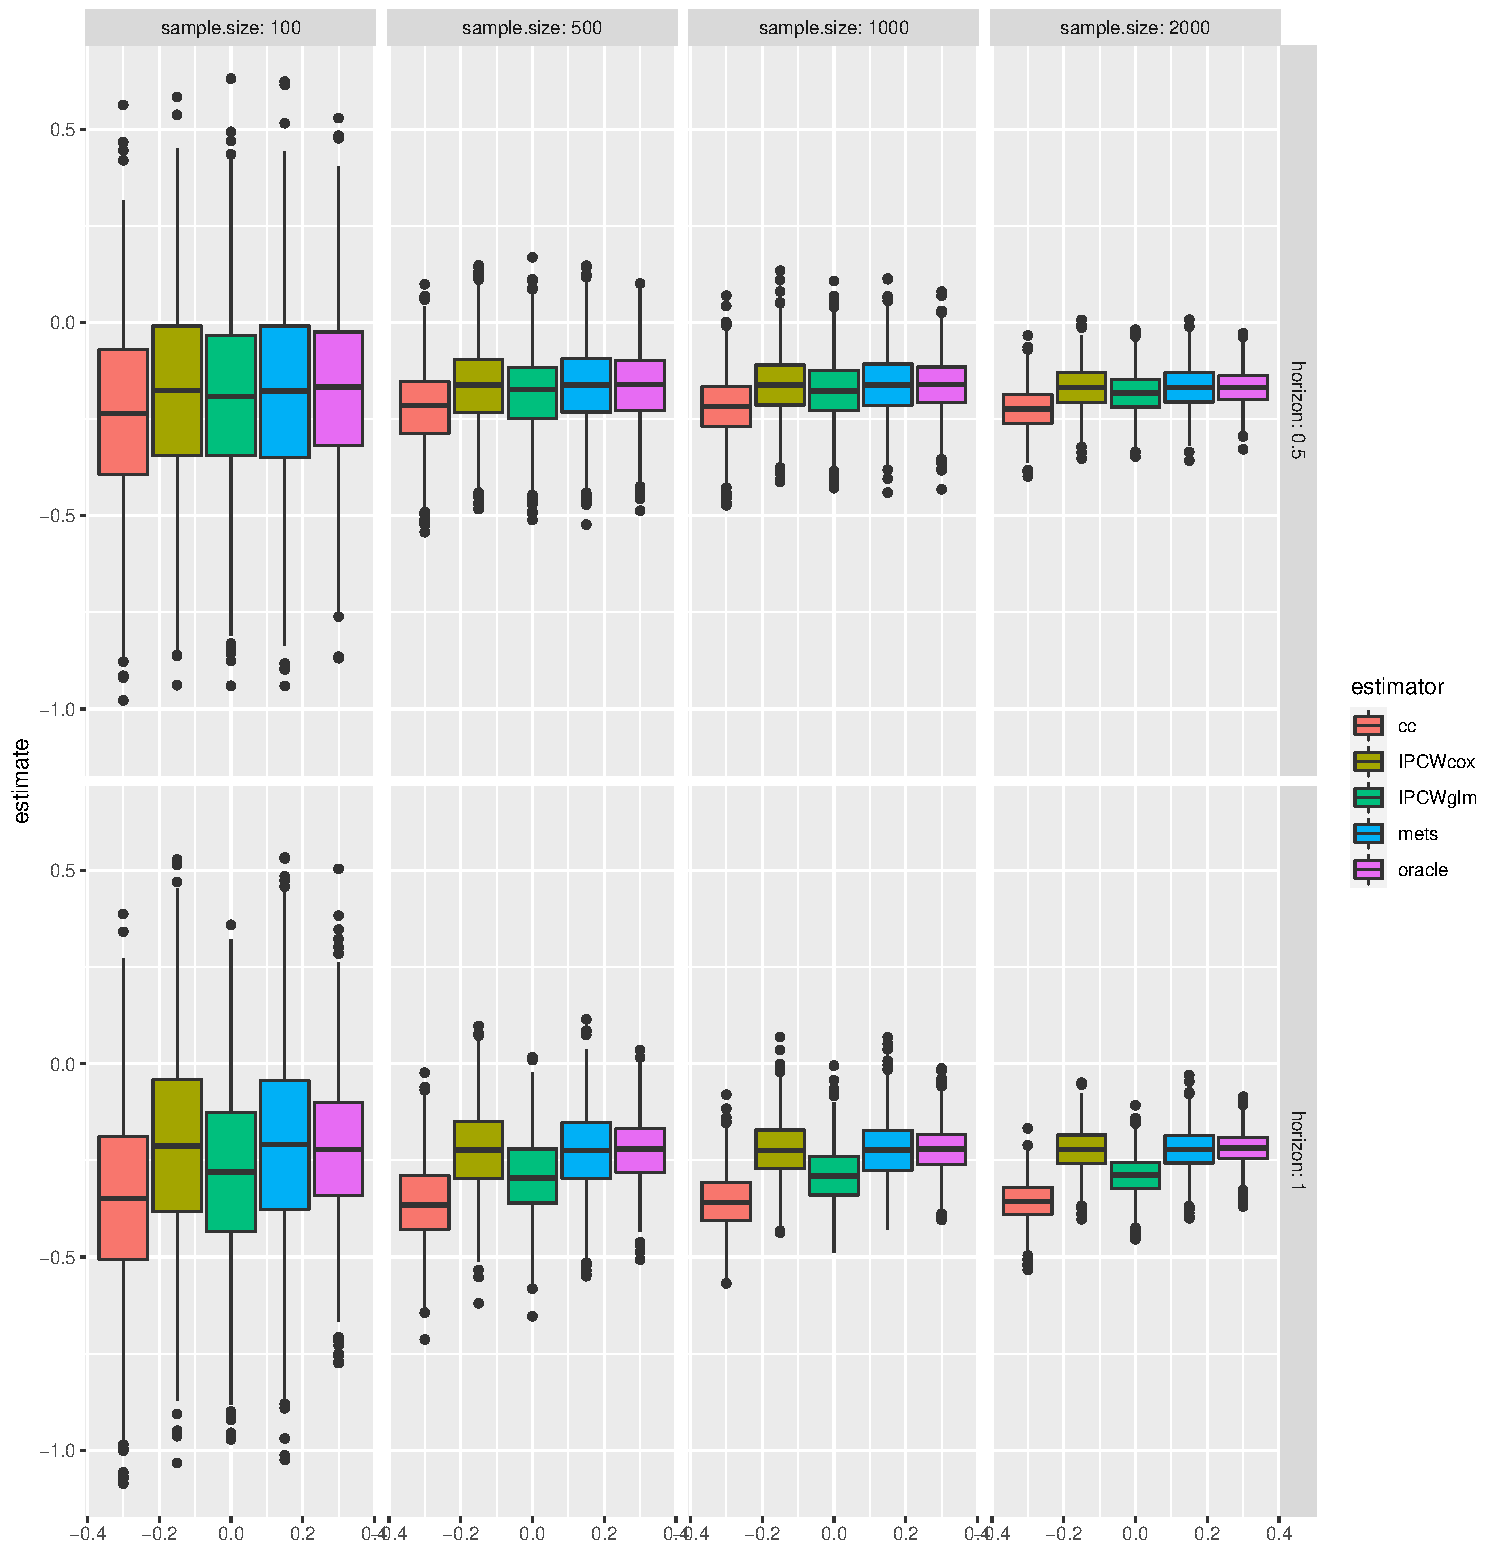
\includegraphics[width=\textwidth]{./figures/simStudy-bin-bias.pdf}
\caption{\label{fig:simulationBinary}Comparison between the empirical distributions of the estimators (binary case) across sample size. Based on 1000 replicates.}
\end{figure}


\appendix
\titleformat{\section}
{\normalfont\Large\bfseries}{}{1em}{Appendix~\thesection:~}

\renewcommand{\thefigure}{\Alph{figure}}
\renewcommand{\thetable}{\Alph{table}}
\renewcommand{\theequation}{\Alph{equation}}

\setcounter{figure}{0}    
\setcounter{table}{0}    
\setcounter{equation}{0}    

\clearpage

\section{Rcode (continuous case)}
\label{sec:org291628f}
\subsection{Generative data model}
\label{SM:datasim}
\lstset{language=r,label= ,caption= ,captionpos=b,numbers=none}
\begin{lstlisting}
simTrialC <- function(n, rho, dmu, causeC, piC,
                      df = Inf, gamma = NULL, unif = NULL){
  
  ## load packages and check user input
  require(mvtnorm)
  require(data.table)
  causeC <- match.arg(causeC, c("random","baseline","latent"))
  
  ## simulate data
  sigma <- 10
  Sigma <- sigma^2*matrix(c(1,rho,rho,1),2,2)

  ## gather into dataset
  if(missing(df) || is.null(df) || is.infinite(df)){
    M.Ym <- rmvnorm(n, mean = c(50, 50-dmu[1]), sigma = Sigma)
    M.Ys <- rmvnorm(n, mean = c(75, 75-dmu[2]), sigma = Sigma)
  }else{
    M.Ym <- rmvt(n, delta = c(50, 50-dmu[1]), sigma = Sigma, df = df)
    M.Ys <- rmvt(n, delta = c(75, 75-dmu[2]), sigma = Sigma, df = df)
  }
  if(!missing(gamma) && !is.null(gamma)){
    M.Ym <- M.Ym + rgamma(2*n, shape = gamma[1], scale = gamma[2])
    M.Ys <- M.Ys + rgamma(2*n, shape = gamma[1], scale = gamma[2])
  }
  if(!missing(unif) && !is.null(unif)){
    M.Ym <- M.Ym + runif(2*n, min = unif[1], max = unif[2])
    M.Ys <- M.Ys + runif(2*n, min = unif[1], max = unif[2])
  }
  dtL <- rbind(
    data.table(id = 1:n, mdd = "moderate", time = "T1", Y = M.Ym[,1]),
    data.table(id = 1:n, mdd = "moderate", time = "T2", Y = M.Ym[,2]),
    data.table(id = n+(1:n), mdd = "severe", time = "T1", Y = M.Ys[,1]),
    data.table(id = n+(1:n), mdd = "severe", time = "T2", Y = M.Ys[,2])
  )
  
  ## define probability of dropout
  dtL$probaDO <- 0
  if(causeC == "random"){
    dtL[time=="T2", probaDO := piC[1]]
  }else if(causeC == "latent"){
    dtL[time=="T2", probaDO := ifelse(.SD$mdd=="moderate",piC[1],piC[2])]
  }else if(causeC == "baseline"){
    dtL$res <- 0
    Ybar <- dtL[time=="T1",mean(Y)]
    dtL[mdd=="moderate", res := c((Y[1]-Ybar)/sigma,NA), by = "id"]
    dtL[mdd=="severe", res := c((Y[1]-Ybar)/sigma,NA), by = "id"]
    dtL[mdd=="moderate", probaDO := c(0,plogis(piC[1]*res[1])), by = "id"]
    dtL[mdd=="severe", probaDO := c(0,plogis(piC[1]*res[1])), by = "id"]
    dtL$res <- NULL 
  }
  
  ## simulate dropout
  dtL[,c("dropout","Yobs") := .(rbinom(.N,prob=probaDO,size=1),Y)]
  dtL[dropout==1,Yobs:=NA]
  
  ## export
  dtL$probaDO <- NULL
  setkeyv(dtL,"id")
  return(dtL)
}
\end{lstlisting}

\subsection{Trial analysis}
\label{SM:dataAnalysis}

\subsection{Multiple trial analysis}
\label{SM:MultipleDataAnalysis}
\lstset{language=r,label= ,caption= ,captionpos=b,numbers=none}
\begin{lstlisting}
warper3TrialC <- function(n, rho, dmu, piC, n.rep = 1,
                          df = Inf, gamma = NULL, unif = NULL,
                          cl = NULL, trace = n.rep>1, short = FALSE, seed = NULL){

  require(pbapply)

  ## normalize arguments
  if(!is.list(piC) || length(piC)!=3){
    stop("Argument \'piC\' should be a list of length 3. \n")
  }
  grid.seed <- expand.grid(rho = rho,
                           rep = 1:n.rep)
  if(length(seed)==1 && NROW(grid.seed)>1){
    set.seed(seed)
    grid.seed$seed <- sample.int(1e6, size = NROW(grid.seed), replace = FALSE)
  }else{
    grid.seed$seed <- seed
  }

  ## internal warper
  .warper3TrialC <- function(iSim){ ## iSim <- 1
    iOut <- NULL
    for(iR in 1:length(rho)){ ## iR <- 1
      iSeed <- grid.seed[grid.seed$rho==rho[iR] & grid.seed$rep == iSim,"seed"]

      iRes <- warperTrialC(n = n, rho = rho[iR], dmu = dmu, causeC = "random", piC = piC[[1]],
                           df = df, gamma = gamma, unif = unif, seed = iSeed)
      if(!inherits(iRes,"try-error")){
        iOut <- rbind(iOut,iRes)
      }    
      iRes <- warperTrialC(n = n, rho = rho[iR], dmu = dmu, causeC = "baseline", piC = piC[[2]],
                           df = df, gamma = gamma, unif = unif, seed = iSeed)
      if(!inherits(iRes,"try-error")){
        iOut <- rbind(iOut,iRes)
      }    
      iRes <- warperTrialC(n = n, rho = rho[iR], dmu = dmu, causeC = "latent", piC = piC[[3]],
                          df = df, gamma = gamma, unif = unif, seed = iSeed)
      if(!inherits(iRes,"try-error")){
        iOut <- rbind(iOut,iRes)
      }    
    }
    return(iOut)
  }
  
  ## iterate
  if(trace==TRUE){
    ls.res <- pblapply(1:n.rep, FUN = .warper3TrialC, cl = cl)
  }else{
    ls.res <- lapply(1:n.rep, FUN = .warper3TrialC)
  }
  out <- do.call(rbind,ls.res)

  ## export
  if(!short){
    out$estimator <-  factor(out$model, c("complete case","FI","FI.oracle","IPCW","IPCW.oracle","oracle"))
    out$correlation <- paste0("correlation = ", out$rho)
    out$cause <- factor(out$causeC,
                        levels = c("random","baseline","latent"),
                        labels = c("dropout: random", "dropout: baseline score","dropout: latent group"))
  }else{
    test.col <- c("causeC","dropout","rho","n","dmu","seed")
    test.duplicated <- duplicated(out[,test.col])
    out[which(test.duplicated),test.col] <- ""
  }
  return(out)

}
\end{lstlisting}

\#+END\textsubscript{SRC}

\subsection{Graphical display of the simulation results}
\label{sec:org8778932}

\lstset{language=r,label= ,caption= ,captionpos=b,numbers=none}
\begin{lstlisting}
ggSimRes <- function(data, plot = TRUE, n.break = 5,
                     size.text = 20, ylim = NULL){
  gg <- ggplot(data, aes(y = estimate))
  gg <- gg + geom_hline(yintercept = median(data[data$model=="oracle","estimate"]), color = "darkgrey", linewidth = 1)
  gg <- gg + geom_boxplot(aes(fill=estimator))
  gg <- gg + facet_grid(cause~correlation)
  gg <- gg + scale_y_continuous(breaks = scales::pretty_breaks(n = n.break))
  if(!is.null(ylim)){
  gg <- gg + coord_cartesian(ylim = ylim)
  }
  gg <- gg + theme(axis.title.x=element_blank(),
                   axis.text.x=element_blank(),
                   axis.ticks.x=element_blank(),
                   text = element_text(size=size.text),
                   axis.line = element_line(linewidth = 1.25),
                   axis.ticks = element_line(size = 2),
                   axis.ticks.length=unit(.25, "cm"),
                   legend.key.size = unit(2,"line"),
                   legend.position="bottom",
                   legend.direction = "horizontal")
  if(plot){print(gg)}
  
  return(invisible(gg))
}
\end{lstlisting}

\subsection{Graphical display of the imputation (\autoref{fig:imputationModel})}
\label{SM:imputation}
Alternative R code to fit a random intercept model
\lstset{language=r,label= ,caption= ,captionpos=b,numbers=none}
\begin{lstlisting}
library(LMMstar)
e.lmm <- lmm(Yobs~time, repetition = ~time|id,
             structure = "CS", data = dtL.B)
eOracle.lmm <- lmm(Yobs~time*mdd, repetition = ~time|id,
                   structure = "CS", data = dtL.B)
\end{lstlisting}

Identify patient with missing data:
\lstset{language=r,label= ,caption= ,captionpos=b,numbers=none}
\begin{lstlisting}
id.NA <- unique(sort(dtL.B[is.na(Yobs),id]))
dtL.BNA <- dtL.B[id %in% id.NA==TRUE]
dtL.BNA$group2 <- paste0(dtL.BNA$mdd," (partially observed)")
dtL.BNNA <- dtL.B[id %in% id.NA==FALSE]
dtL.BNNA$group2 <- paste0(dtL.BNNA$mdd," (fully observed)")
\end{lstlisting}

Identify patient with missing data and get the imputed value
\lstset{language=r,label= ,caption= ,captionpos=b,numbers=none}
\begin{lstlisting}
pred.B <- predict(e.lmm, newdata = dtL.BNA, type = "dynamic",
                  keep.newdata = TRUE)
pred.B$mdd <- paste(pred.B$mdd," (imputed)")
predOracle.B <- predict(eOracle.lmm, newdata = dtL.BNA, type = "dynamic",
                        keep.newdata = TRUE)
predOracle.B$mdd <- paste(predOracle.B$mdd," (imputed)")
\end{lstlisting}

Mixed model (feasible) estimate as a t-test on the imputed values:
\lstset{language=r,label= ,caption= ,captionpos=b,numbers=none}
\begin{lstlisting}
diff.lmm <- c(dtL.BNNA[,diff(Yobs),by="id"][[2]],
              pred.B[,estimate[2]-Yobs[1],by="id"][[2]])
t.test(diff.lmm)
coef(e.lmm)["timeT2"]
\end{lstlisting}

\begin{verbatim}

	One Sample t-test

data:  diff.lmm
t = -149.14, df = 1999, p-value < 2.2e-16
alternative hypothesis: true mean is not equal to 0
95 percent confidence interval:
 -35.17796 -34.26483
sample estimates:
mean of x 
-34.72139
   timeT2 
-34.72139
\end{verbatim}

Mixed model (oracle) estimate as a t-test on the imputed values:
\lstset{language=r,label= ,caption= ,captionpos=b,numbers=none}
\begin{lstlisting}
diff.lmm.oracle <- c(dtL.BNNA[,diff(Yobs),by="id"][[2]],
                     predOracle.B[,estimate[2]-Yobs[1],by="id"][[2]])
t.test(diff.lmm.oracle)
glht(eOracle.lmm, linfct = "timeT2+0.5*timeT2:mddsevere=0")

\end{lstlisting}

\begin{verbatim}

	One Sample t-test

data:  diff.lmm.oracle
t = -125.01, df = 1999, p-value < 2.2e-16
alternative hypothesis: true mean is not equal to 0
95 percent confidence interval:
 -38.02137 -36.84682
sample estimates:
mean of x 
 -37.4341

	 General Linear Hypotheses

Linear Hypotheses:
                                     Estimate
timeT2 + 0.5 * timeT2:mddsevere == 0   -37.43
\end{verbatim}

Graphical display (feasible):
\lstset{language=r,label= ,caption= ,captionpos=b,numbers=none}
\begin{lstlisting}
gg.imp <- ggplot(mapping = aes(x=time, color = group2))
gg.imp <- gg.imp + geom_boxplot(data = dtL.BNNA, mapping = aes(y = Yobs))
gg.imp <- gg.imp + geom_boxplot(data = dtL.BNA, mapping = aes(y = Yobs))
gg.imp <- gg.imp + geom_boxplot(data = pred.B, mapping = aes(y = estimate))
gg.imp <- gg.imp + scale_color_manual("MDD group",
                                      values = c("limegreen","darkgreen","orange","red"))
gg.imp <- gg.imp + theme(text = element_text(size=15),
                         axis.line = element_line(size = 1.25),
                         axis.ticks = element_line(size = 2),
                         axis.ticks.length=unit(.25, "cm"),
                         legend.position="bottom",
                         legend.direction = "horizontal")
gg.imp
\end{lstlisting}

\begin{verbatim}
Advarselsbeskeder:
1: Removed 969 rows containing non-finite values (stat_boxplot). 
2: Removed 969 rows containing non-finite values (stat_boxplot).
\end{verbatim}


Graphical display (oracle):
\lstset{language=r,label= ,caption= ,captionpos=b,numbers=none}
\begin{lstlisting}
gg.impOracle <- ggplot(mapping = aes(x=time, color = group2))
gg.impOracle <- gg.impOracle + geom_boxplot(data = dtL.BNNA, mapping = aes(y = Yobs))
gg.impOracle <- gg.impOracle + geom_boxplot(data = dtL.BNA, mapping = aes(y = Yobs))
gg.impOracle <- gg.impOracle + geom_boxplot(data = predOracle.B, mapping = aes(y = estimate))
gg.impOracle <- gg.impOracle + scale_color_manual("MDD group",
                                      values = c("limegreen","darkgreen","orange","red"))
gg.impOracle <- gg.impOracle + theme(text = element_text(size=15),
                         axis.line = element_line(size = 1.25),
                         axis.ticks = element_line(size = 2),
                         axis.ticks.length=unit(.25, "cm"),
                         legend.position="bottom",
                         legend.direction = "horizontal")
gg.impOracle
\end{lstlisting}

\begin{verbatim}
Advarselsbeskeder:
1: Removed 969 rows containing non-finite values (stat_boxplot). 
2: Removed 969 rows containing non-finite values (stat_boxplot).
\end{verbatim}
\end{document}